\documentclass[a4paper,12pt,twoside]{memoir}

% Castellano
\usepackage[spanish,es-tabla]{babel}
\selectlanguage{spanish}
\usepackage[utf8]{inputenc}
\usepackage[T1]{fontenc}
\usepackage{lmodern} % scalable font
\usepackage{microtype}
\usepackage{placeins}

\usepackage[numbers,sort]{natbib}

\RequirePackage{booktabs}
\RequirePackage[table]{xcolor}
\RequirePackage{xtab}
\RequirePackage{multirow}
\RequirePackage{longtable}

% Links
\PassOptionsToPackage{hyphens}{url}\usepackage[colorlinks]{hyperref}
\hypersetup{
	allcolors = {red}
}

% Ecuaciones
\usepackage{amsmath}
\usepackage{eurosym}

% Rutas de fichero / paquete
\newcommand{\ruta}[1]{{\sffamily #1}}

% Párrafos
\nonzeroparskip

% Huérfanas y viudas
\widowpenalty100000
\clubpenalty100000

% Evitar solapes en el header
\nouppercaseheads

% Imagenes
\usepackage{graphicx}
\usepackage{subcaption}
\newcommand{\imagen}[2]{
	\begin{figure}[!h]
		\centering
		\includegraphics[width=0.9\textwidth]{#1}
		\caption{#2}\label{fig:#1}
	\end{figure}
	\FloatBarrier
}

\newcommand{\imagenflotante}[2]{
	\begin{figure}%[!h]
		\centering
		\includegraphics[width=0.9\textwidth]{#1}
		\caption{#2}\label{fig:#1}
	\end{figure}
}



% El comando \figura nos permite insertar figuras comodamente, y utilizando
% siempre el mismo formato. Los parametros son:
% 1 -> Porcentaje del ancho de página que ocupará la figura (de 0 a 1)
% 2 --> Fichero de la imagen
% 3 --> Texto a pie de imagen
% 4 --> Etiqueta (label) para referencias
% 5 --> Opciones que queramos pasarle al \includegraphics
% 6 --> Opciones de posicionamiento a pasarle a \begin{figure}
\newcommand{\figuraConPosicion}[6]{%
  \setlength{\anchoFloat}{#1\textwidth}%
  \addtolength{\anchoFloat}{-4\fboxsep}%
  \setlength{\anchoFigura}{\anchoFloat}%
  \begin{figure}[#6]
    \begin{center}%
      \Ovalbox{%
        \begin{minipage}{\anchoFloat}%
          \begin{center}%
            \includegraphics[width=\anchoFigura,#5]{#2}%
            \caption{#3}%
            \label{#4}%
          \end{center}%
        \end{minipage}
      }%
    \end{center}%
  \end{figure}%
}

%
% Comando para incluir imágenes en formato apaisado (sin marco).
\newcommand{\figuraApaisadaSinMarco}[5]{%
  \begin{figure}%
    \begin{center}%
    \includegraphics[angle=90,height=#1\textheight,#5]{#2}%
    \caption{#3}%
    \label{#4}%
    \end{center}%
  \end{figure}%
}
% Para las tablas
\newcommand{\otoprule}{\midrule [\heavyrulewidth]}
%
% Nuevo comando para tablas pequeñas (menos de una página).
\newcommand{\tablaSmall}[5]{%
 \begin{table}
  \begin{center}
   \rowcolors {2}{gray!35}{}
   \begin{tabular}{#2}
    \toprule
    #4
    \otoprule
    #5
    \bottomrule
   \end{tabular}
   \caption{#1}
   \label{tabla:#3}
  \end{center}
 \end{table}
}

%
%Para el float H de tablaSmallSinColores
\usepackage{float}

%
% Nuevo comando para tablas pequeñas (menos de una página).
\newcommand{\tablaSmallSinColores}[5]{%
 \begin{table}[H]
  \begin{center}
   \begin{tabular}{#2}
    \toprule
    #4
    \otoprule
    #5
    \bottomrule
   \end{tabular}
   \caption{#1}
   \label{tabla:#3}
  \end{center}
 \end{table}
}

\newcommand{\tablaApaisadaSmall}[5]{%
\begin{landscape}
  \begin{table}
   \begin{center}
    \rowcolors {2}{gray!35}{}
    \begin{tabular}{#2}
     \toprule
     #4
     \otoprule
     #5
     \bottomrule
    \end{tabular}
    \caption{#1}
    \label{tabla:#3}
   \end{center}
  \end{table}
\end{landscape}
}

%
% Nuevo comando para tablas grandes con cabecera y filas alternas coloreadas en gris.
\newcommand{\tabla}[6]{%
  \begin{center}
    \tablefirsthead{
      \toprule
      #5
      \otoprule
    }
    \tablehead{
      \multicolumn{#3}{l}{\small\sl continúa desde la página anterior}\\
      \toprule
      #5
      \otoprule
    }
    \tabletail{
      \hline
      \multicolumn{#3}{r}{\small\sl continúa en la página siguiente}\\
    }
    \tablelasttail{
      \hline
    }
    \bottomcaption{#1}
    \rowcolors {2}{gray!35}{}
    \begin{xtabular}{#2}
      #6
      \bottomrule
    \end{xtabular}
    \label{tabla:#4}
  \end{center}
}

%
% Nuevo comando para tablas grandes con cabecera.
\newcommand{\tablaSinColores}[6]{%
  \begin{center}
    \tablefirsthead{
      \toprule
      #5
      \otoprule
    }
    \tablehead{
      \multicolumn{#3}{l}{\small\sl continúa desde la página anterior}\\
      \toprule
      #5
      \otoprule
    }
    \tabletail{
      \hline
      \multicolumn{#3}{r}{\small\sl continúa en la página siguiente}\\
    }
    \tablelasttail{
      \hline
    }
    \bottomcaption{#1}
    \begin{xtabular}{#2}
      #6
      \bottomrule
    \end{xtabular}
    \label{tabla:#4}
  \end{center}
}

%
% Nuevo comando para tablas grandes sin cabecera.
\newcommand{\tablaSinCabecera}[5]{%
  \begin{center}
    \tablefirsthead{
      \toprule
    }
    \tablehead{
      \multicolumn{#3}{l}{\small\sl continúa desde la página anterior}\\
      \hline
    }
    \tabletail{
      \hline
      \multicolumn{#3}{r}{\small\sl continúa en la página siguiente}\\
    }
    \tablelasttail{
      \hline
    }
    \bottomcaption{#1}
  \begin{xtabular}{#2}
    #5
   \bottomrule
  \end{xtabular}
  \label{tabla:#4}
  \end{center}
}



\definecolor{cgoLight}{HTML}{EEEEEE}
\definecolor{cgoExtralight}{HTML}{FFFFFF}

%
% Nuevo comando para tablas grandes sin cabecera.
\newcommand{\tablaSinCabeceraConBandas}[5]{%
  \begin{center}
    \tablefirsthead{
      \toprule
    }
    \tablehead{
      \multicolumn{#3}{l}{\small\sl continúa desde la página anterior}\\
      \hline
    }
    \tabletail{
      \hline
      \multicolumn{#3}{r}{\small\sl continúa en la página siguiente}\\
    }
    \tablelasttail{
      \hline
    }
    \bottomcaption{#1}
    \rowcolors[]{1}{cgoExtralight}{cgoLight}

  \begin{xtabular}{#2}
    #5
   \bottomrule
  \end{xtabular}
  \label{tabla:#4}
  \end{center}
}




\graphicspath{ {./img/} }

% Capítulos
\chapterstyle{bianchi}
\newcommand{\capitulo}[2]{
	\setcounter{chapter}{#1}
	\setcounter{section}{0}
	\setcounter{figure}{0}
	\setcounter{table}{0}
	\chapter*{#2}
	\addcontentsline{toc}{chapter}{#2}
	\markboth{#2}{#2}
}

% Apéndices
\renewcommand{\appendixname}{Apéndice}
\renewcommand*\cftappendixname{\appendixname}

\newcommand{\apendice}[1]{
	%\renewcommand{\thechapter}{A}
	\chapter{#1}
}

\renewcommand*\cftappendixname{\appendixname\ }

% Formato de portada
\makeatletter
\usepackage{xcolor}
\newcommand{\tutor}[1]{\def\@tutor{#1}}
\newcommand{\course}[1]{\def\@course{#1}}
\definecolor{cpardoBox}{HTML}{E6E6FF}
\def\maketitle{
  \null
  \thispagestyle{empty}
  % Cabecera ----------------
\noindent
\includegraphics[width=\textwidth]{cabecera}\vspace{1cm}%
  \vfill
  % Título proyecto y escudo informática ----------------
  \colorbox{cpardoBox}{%
    \begin{minipage}{.8\textwidth}
      \vspace{.5cm}\Large
      \begin{center}
      \textbf{TFG del Grado en Ingeniería Informática}\vspace{.6cm}\\
      \textbf{\LARGE\@title{}}
      \end{center}
      \vspace{.2cm}
    \end{minipage}

  }%
  \hfill\begin{minipage}{.20\textwidth}
    
\includegraphics[width=\textwidth]{escudoInfor}
  \end{minipage}
  \vfill
  % Datos de alumno, curso y tutores ------------------
  \begin{center}%
  {%
    \noindent\LARGE
    Presentado por \@author{}\\ 
    Universidad de Burgos \\ \@date{}\\
    Tutor: \@tutor{}\\
  }%
  \end{center}%
  \null
  \cleardoublepage
  }
\makeatother


% Datos de portada
\title{GII\_O\_MA\_19.07 \\Comparador de métricas de evolución en repositorios Software \\Documentación Técnica}
\author{Joaquín García Molina}
\tutor{Carlos López Nozal}
\date{\today}

\begin{document}

\maketitle



\cleardoublepage



%%%%%%%%%%%%%%%%%%%%%%%%%%%%%%%%%%%%%%%%%%%%%%%%%%%%%%%%%%%%%%%%%%%%%%%%%%%%%%%%%%%%%%%%



\frontmatter


\clearpage

% Indices
\tableofcontents

\clearpage

\listoffigures

\clearpage

\listoftables

\clearpage

\mainmatter

\appendix

\apendice{Plan de Proyecto Software}\label{anex:A}

\section{Introducción}

Lo primero que se debería hacer al iniciar un proyecto y antes de comenzar con el desarrollo es la planificación del mismo. Es necesario realizar una estimación de coste en tiempo y dinero que nos va a suponer realizar el proyecto y una vez conozcamos esta estimación deducir si el proyecto se puede realizar exitosamente o no. 
Para realizar esta tarea en este documento vamos a realizar dos tareas:

\begin{description}
	\tightlist
	\item[Planificación temporal.] Donde estimaremos el tiempo que requiere la realización del proyecto.
	\item[Estudio de la viabilidad.] Donde se deduce si el proyecto es viable, tanto económica como legalmente: 
	\begin{description}
		\tightlist
		\item[Viabilidad económica.] Se estudia el coste que supondría haber realizado el proyecto en un entorno real y se analizan posibles maneras de monetizar el proyecto para cubrir este coste.
		\item[Viabilidad legal.] Se estudian las leyes aplicables al proyecto y los aspectos más relevantes a nivel legal.
	\end{description}
\end{description}

\section{Planificación temporal}

Se ha optado por la metodología \textbf{SCRUM} \cite{scrum_master_scrum_2019}, donde se trabaja con un ciclo de vida que se repite durante el proyecto. Trabajar con esta metodología ha significado que:
\begin{itemize}
	\item Se ha trabajado de manera incremental y evolutiva.
	\item Se han trabajado en iteraciones (llamados \textit{sprints} en la metodología \textbf{\textit{SCRUM}}) de dos semanas. Estos \textit{sprints} finalizan con una reunión entre el tutor y alumno donde:
	\begin{itemize}
		\item Se llevaba a cabo la \textit{sprint review}, donde se revisa el trabajo realizado durante el \textit{sprint} que finaliza y se tratan los avances realizados así como los problemas con los que el alumno se ha encontrado.
				\item Una segunda parte donde se lleva a cabo la \textit{sprint planning}, donde se planifica el trabajo a realizar durante el siguiente \textit{sprint} planteando tareas y seleccionándolas del \textit{product backlog}, pasándolas a la pila de trabajo del \textit{sprint} que comienza, el \textit{sprint backlog}.\\
				Estas tareas se han registrado en el sistema de gestión de incidencias de \textit{GitHub} , \textit{GitHub Issues} \footnote{Planificación de proyectos para desarrolladores - \url{https://github.com/features/issues}} y el trabajo con \textit{sprints} se ha llevado a cabo a través de \textit{ZenHub} \footnote{Página de inicio de \textit{ZenHub} - \url{https://www.zenhub.com/}} integrado directamente en \textit{GitHub}.
	\end{itemize}
\end{itemize}

\subsection{\textit{Sprints} realizados}

Además de la división del desarrollo del proyecto en \textit{sprints}, podemos dividirlo en diferentes fases:


\begin{itemize}
	\item Durante la primera fase se llevaron a cabo tareas de \textbf{investigación} y \textbf{estudio} del proyecto previo\cite{TFGPrevio} así como de las bases teóricas y herramientas que se utilizarían durante el proceso.
	
	\item En la segunda fase, una vez comprendidos los conceptos planteados en el proyecto ya existente y en las bases teóricas (métricas, \textit{framework}  de medición, estructura del proyecto, etc.) se realizaron tareas de \textbf{configuración} del entorno de desarrollo, tanto para el código como para la memoria del proyecto.
	
	\item Tercera fase donde gracias a la investigación y estudio realizados se realizan diferentes tareas de \textbf{documentación} de la memoria del proyecto.
	
	\item Cuarta fase, la más extensa de todas, donde se realizan tareas de \textbf{desarrollo} para actualizar las dependencias del proyecto, implementar nuevas métricas, mejoras en la interfaz y la integración con \textit{GitHub}.
	
	\item Quinta fase final de \textbf{documentación} en la que se finaliza la memoria y se trabaja en los anexos. Finalmente se preparan los vídeos necesarios y las guías de usuario.
\end{itemize}

En la siguiente sección se van a describir estas fases, que se pueden también consultar a través de las \textit{issues} del repositorio del proyecto:\\

\url{https://github.com/Joaquin-GM/GII_O_MA_19.07-Comparador-de-metricas-de-evolucion-en-repositorios-Software} \\

Se utilizarán de manera explicativa capturas de la gestión de los \textit{sprints} gestionados con \textit{ZenHub}.



\subsubsection{Investigación y estudio}

Esta fase inicial comenzó en octubre de 2021 y duró aproximadamente 3 \textit{sprints} (6 semanas) durante los que se asentó la base teórica del proyecto y se comprendió la estructura del mismo así como los objetivos. Además del trabajo con las referencias teóricas como \cite{ratzinger_space:_2007} se buscó información sobre trabajos y aplicaciones que están relacionados con la temática de este proyecto ya entreviéndose que hay muy pocas soluciones similares y ninguna con las capacidades que tendría el proyecto a su finalización.\\
También se realizó la formación en \textit{Vaadin} que proponen los propios creadores del \textit{framework} \footnote{Centro de aprendizaje de \textit{Vaadin} - \url{https://vaadin.com/learn/tutorials?version=v14}} así como tutoriales para que el alumno se familiarizara con \textit{LaTeX} y con la herramienta utilizada \textit{TexMaker}\footnote{\textit{TexMaker} editor \textit{LaTeX} - \url{https://www.xm1math.net/texmaker/}}.\\

A continuación se muestran algunas de las \textit{issues} con las que se trabajó en esta fase:

\begin{figure}[!h]
	\centering
	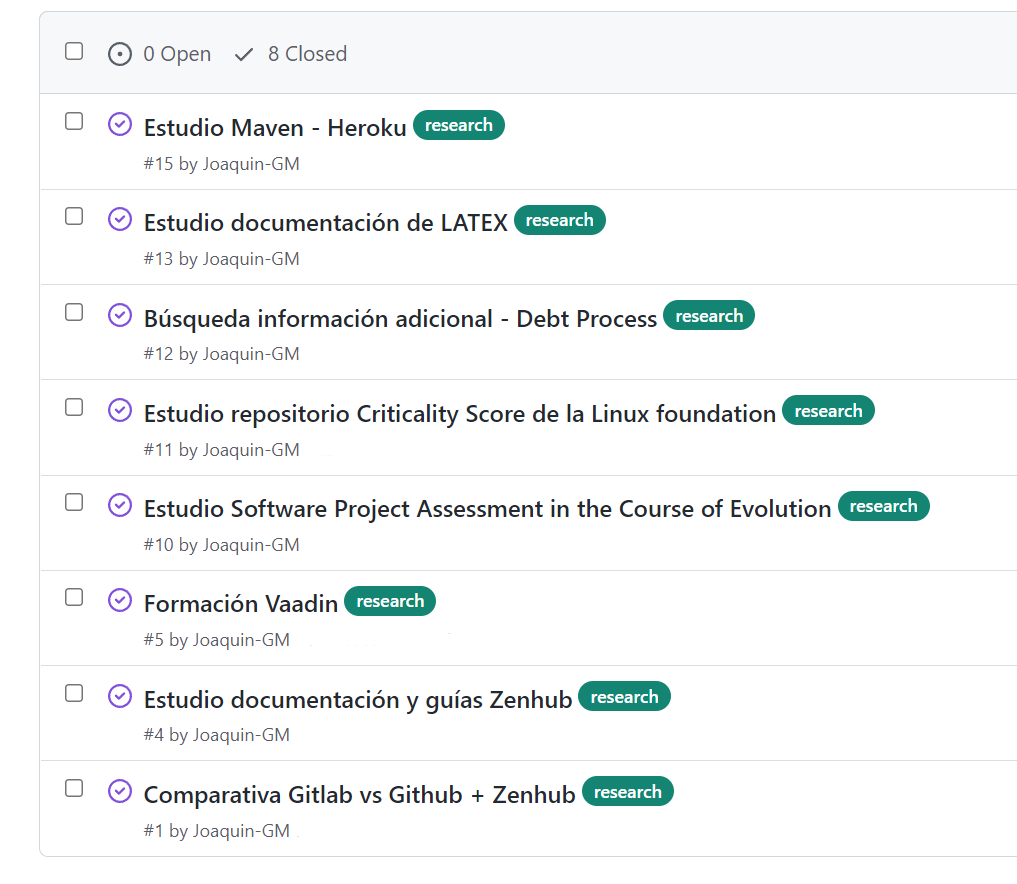
\includegraphics[scale=0.50]{AnexA_Research_Issues}
	\caption{\textit{Issues} relacionadas con la fase de estudio e investigación investigación}
	\label{fig:AnexA_Research_Issues}
\end{figure}
\FloatBarrier

\subsubsection{Configuración del entorno de desarrollo}

En esta fase se trabajó configurando las diferentes herramientas que se iban a utilizar en el proyecto, \textit{GitHub} + \textit{ZenHub} para la gestión de \textit{issues} y \textit{sprints}, Eclipse como \textit{IDE} de desarrollo, \textit{Maven} y \textit{Jetty} para la gestión y ejecución del proyecto en local y \textit{TexMaker} como editor \textit{LaTeX} para trabajar con la memoria. Esta fase duró otros tres \textit{sprints} (6 semanas) y a continuación se muestran las las \textit{issues} con las que se trabajó en esta fase:

\begin{figure}[!h]
	\centering
	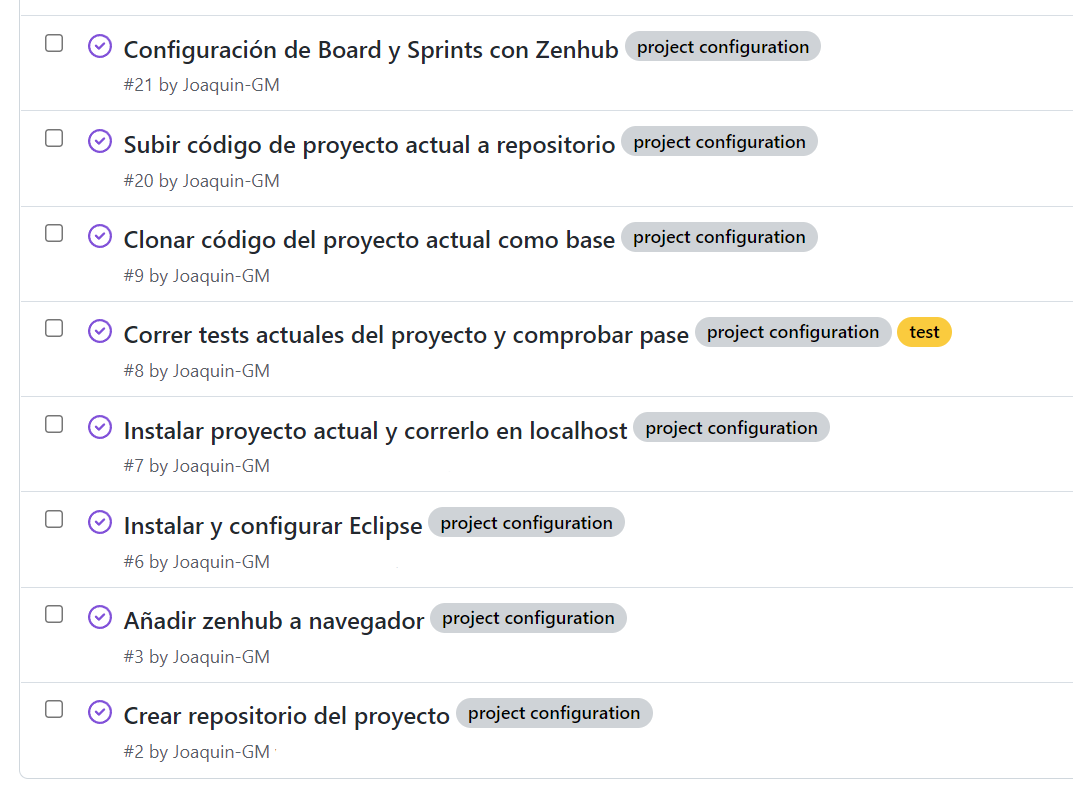
\includegraphics[scale=0.50]{AnexA_Configuration_Issues}
	\caption{\textit{Board} del proyecto en \textit{ZenHub}}
	\label{fig:AnexA_Configuration_Issues}
\end{figure}
\FloatBarrier

También se muestra en la figura \ref{fig:AnexA_Zenhub_Board} cómo quedó el tablero de \textit{ZenHub} una vez estuvo integrado en el repositorio directamente en \textit{GitHub} a través de la extensión de navegador de \textit{ZenHub}:

\begin{figure}[!h]
	\centering
	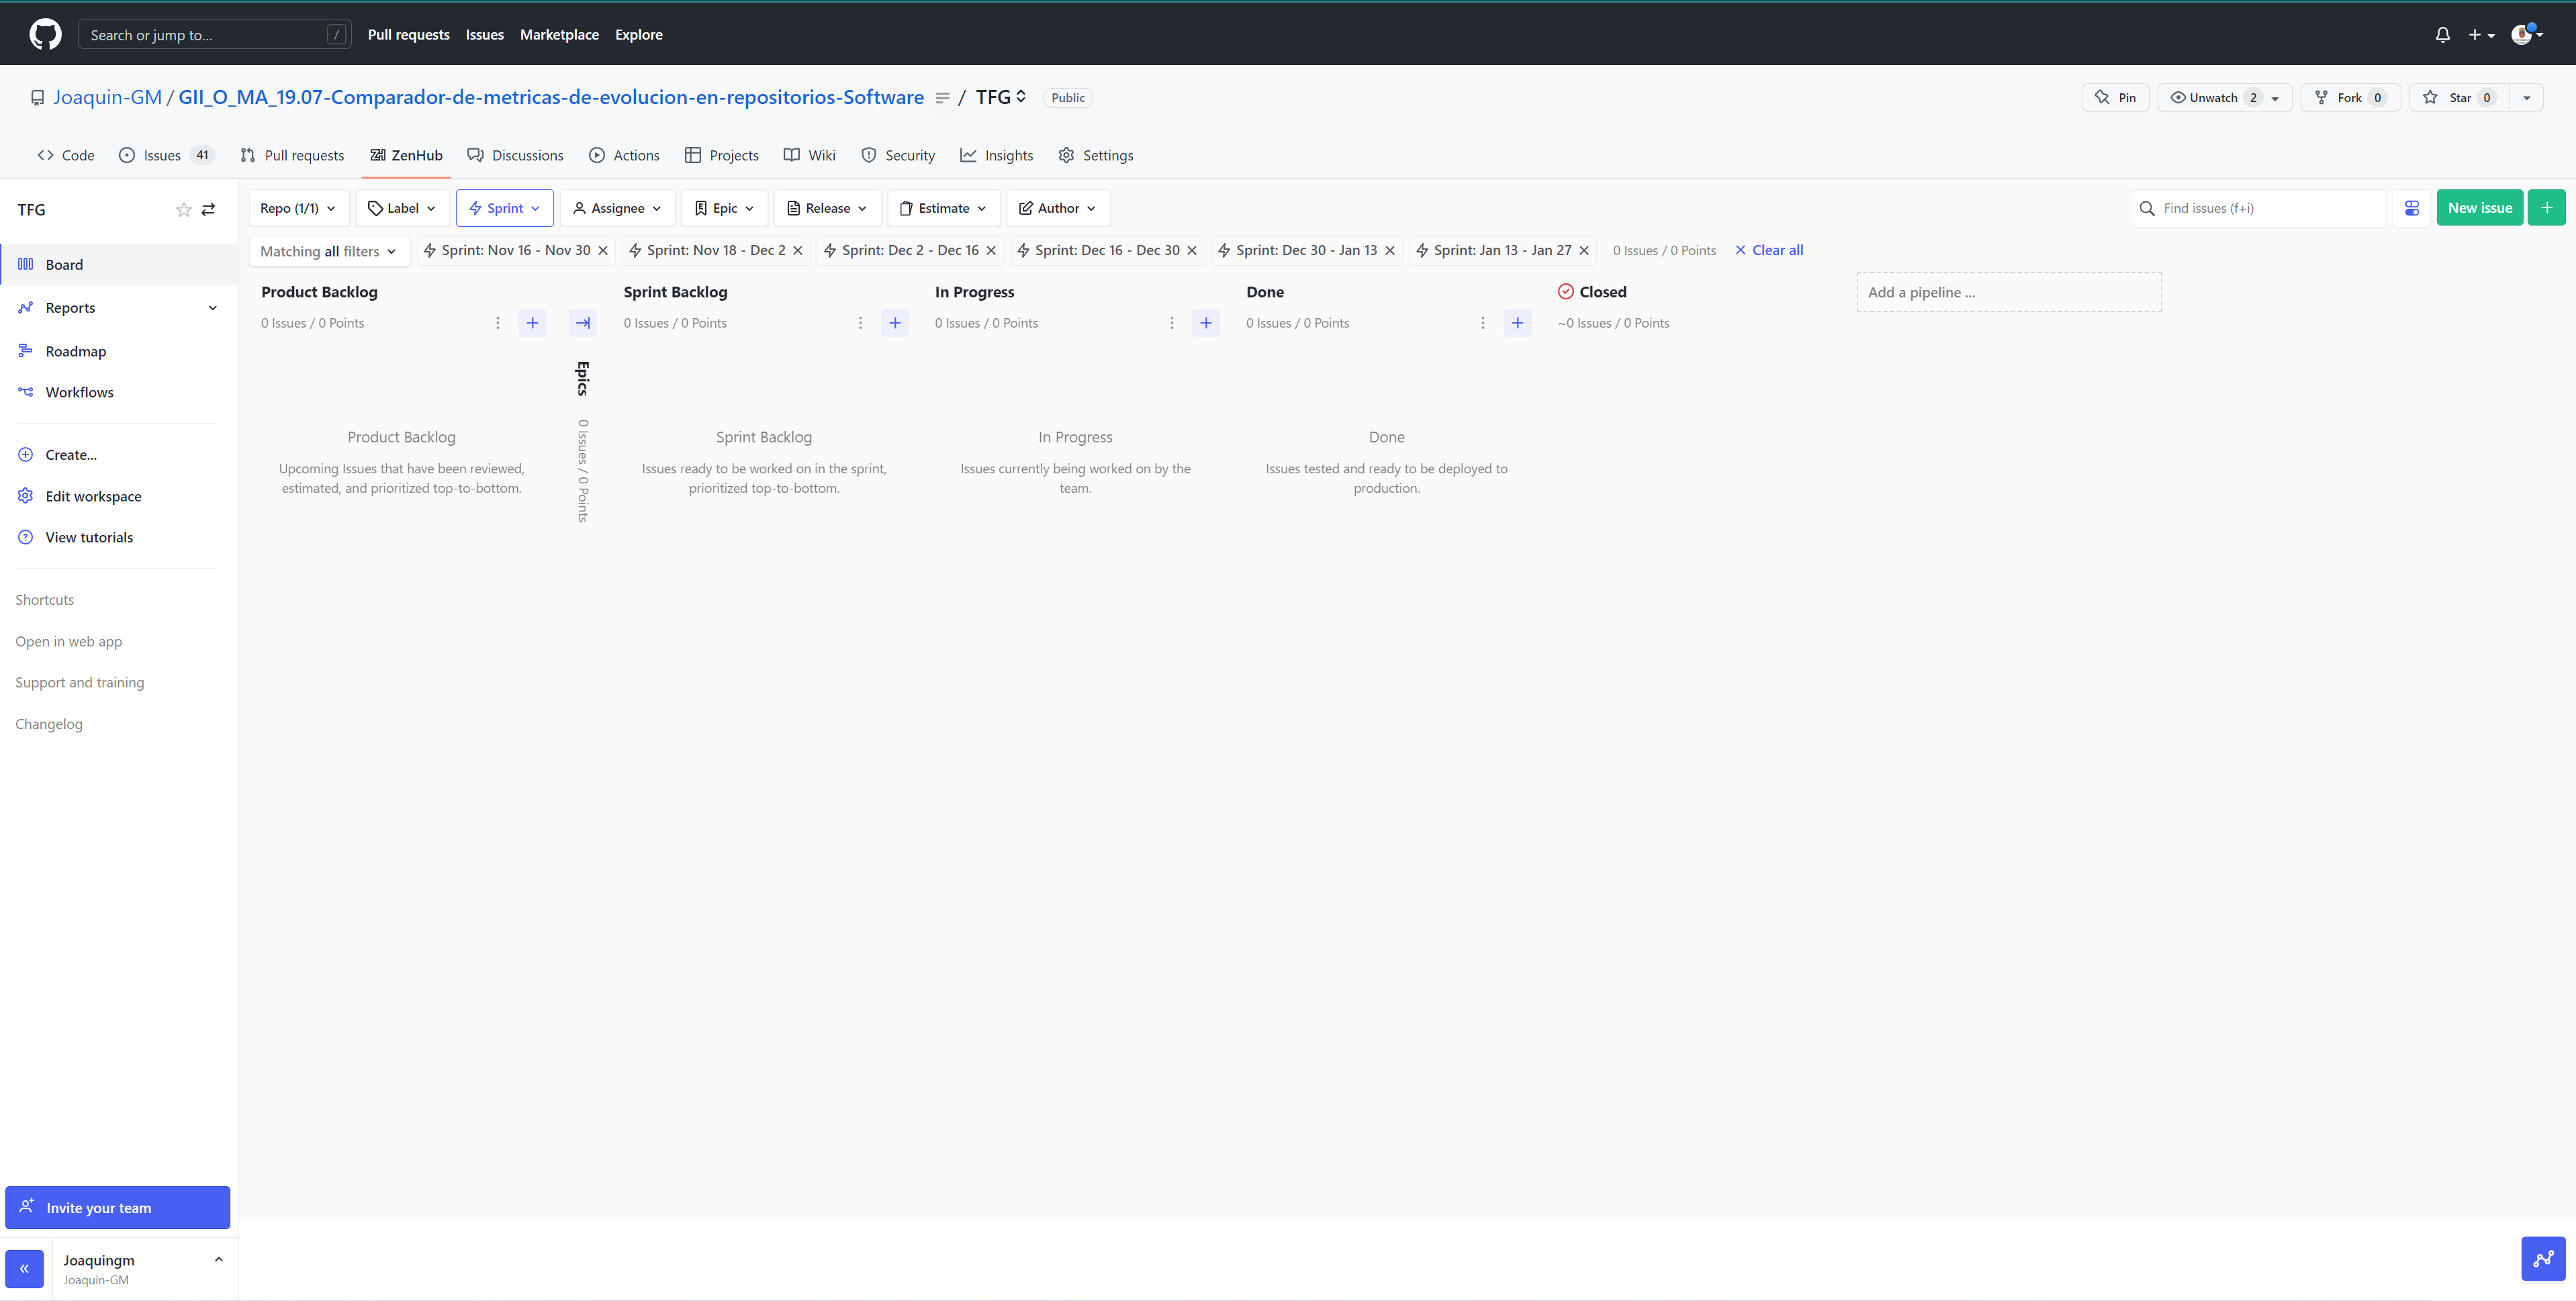
\includegraphics[width=1\textwidth]{AnexA_Zenhub_Board}
	\caption{Creación de nueva \textit{issue} en \textit{ZenHub}}
	\label{fig:AnexA_Zenhub_Board}
\end{figure}
\FloatBarrier

Como se puede apreciar en la figura \ref{fig:AnexA_Zenhub_Board}, \textit{ZenHub} provee de numerosas herramientas muy útiles para la gestión de las \textit{issues} del proyecto permitiéndonos trabajar con ellas de forma sencilla y agruparlas en \textit{sprints}.\\
Para facilitar la creación de nuevas \textit{issues} se crearon plantillas que se pueden utilizar también desde el menú de creación de \textit{issues} de \textit{ZenHub} como se puede ver en la figura \ref{fig:AnexA_Zenhub_Create_New_Issue}

\begin{figure}[!h]
	\centering
	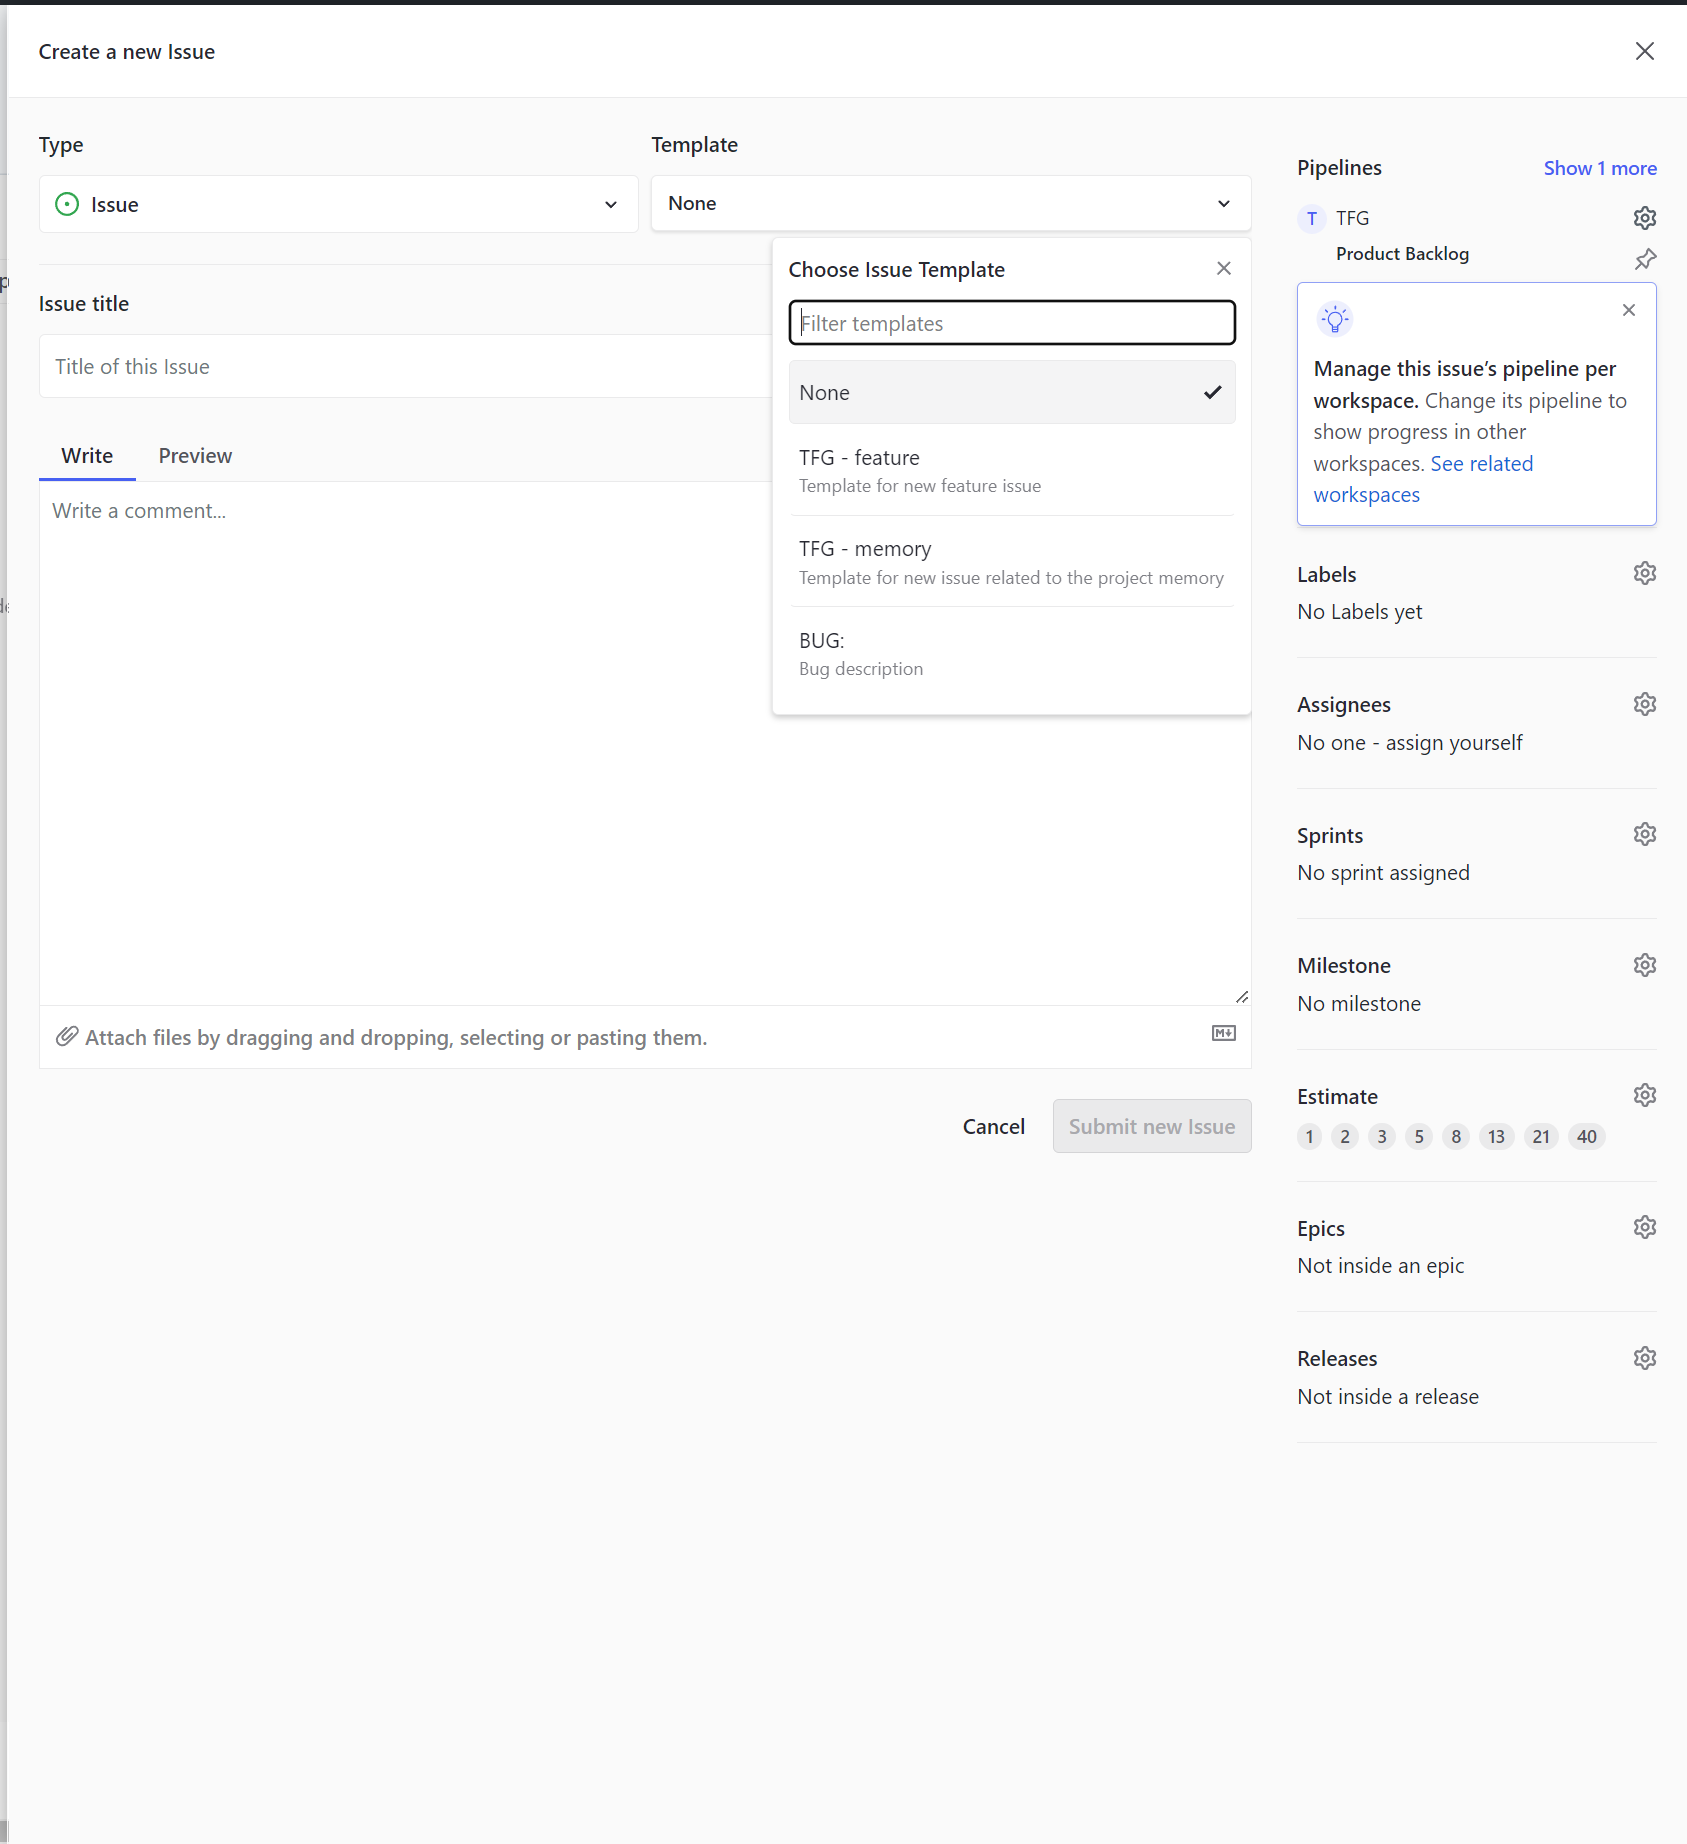
\includegraphics[width=1\textwidth]{AnexA_Zenhub_Create_New_Issue}
	\caption{Creación de nueva \textit{issue} en \textit{ZenHub}}
	\label{fig:AnexA_Zenhub_Create_New_Issue}
\end{figure}
\FloatBarrier

\subsubsection{Primera fase de documentación}

En esta primera fase de documentación se trabajó durante 3 \textit{sprints} (6 semanas) en los siguientes apartados de la memoria:

\begin{itemize}
	\item Introducción y Objetivos
	\item Resumen y Descriptores
	\item Conceptos teóricos
	\item Técnicas y herramientas
	\item Aspectos relevantes del desarrollo del proyecto (que se finalizaría más adelante)
\end{itemize}

A continuación podemos ver las \textit{issues} con las que se trabajó en esta fase:

\begin{figure}[!h]
	\centering
	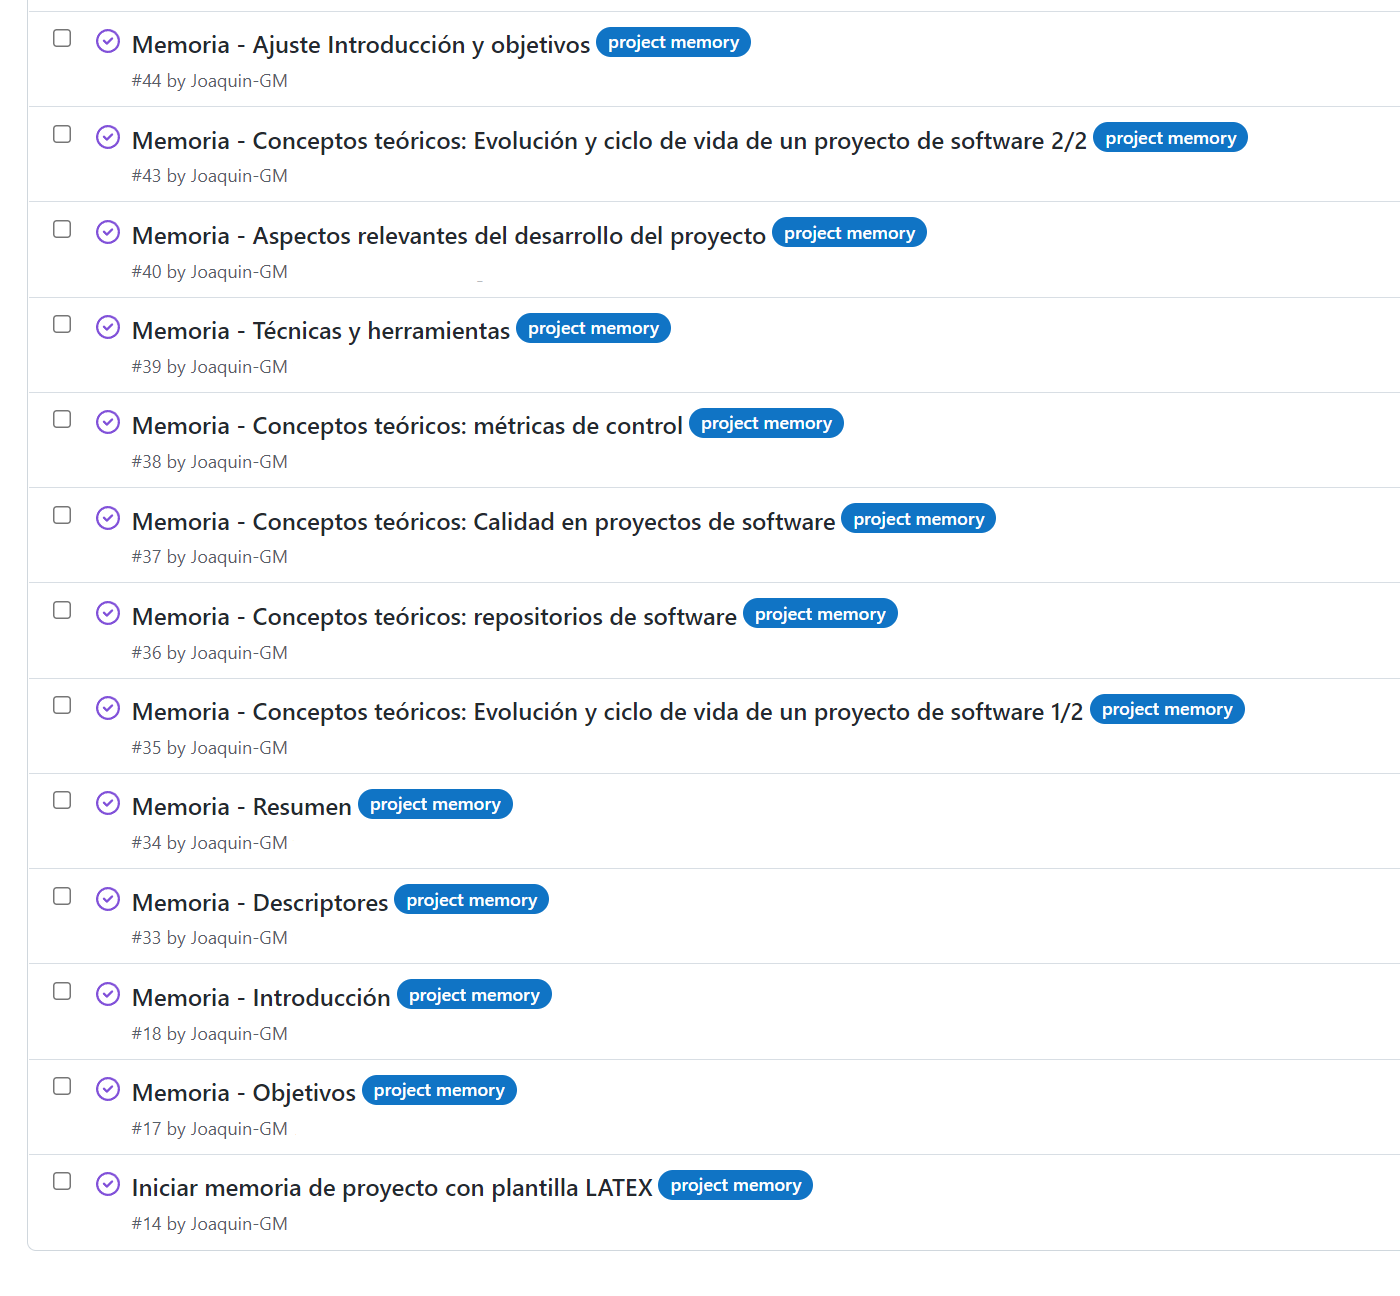
\includegraphics[width=1\textwidth]{AnexA_First_Memory_Issues}
	\caption{Primeras \textit{issues} relacionadas con la memoria}
	\label{fig:AnexA_First_Memory_Issues}
\end{figure}
\FloatBarrier

\textit{ZenHub} también nos proporciona información sobre la gestión de las \textit{issues} y el avance del proyecto. Podemos destacar los gráficos \textit{burndown} que representan el avance durante el transcurso del sprint, marcando una guía orientativa de cómo debería ser. Este tipo de gráfico representa los puntos asignados a las diferentes \textit{issues} y va bajando conforme éstas se van cerrando durante el \textit{sprint}. \\
Como vemos en la figura \ref{fig:AnexA_First_Memory_BurnDown}, en algunos \textit{sprints} se estimó demasiado trabajo o bien no se pudo realizar al completo y en el siguiente gráfico se puede ver cómo no se llegan a completar todos los puntos de las \textit{issues} planteadas:

\begin{figure}[!h]
	\centering
	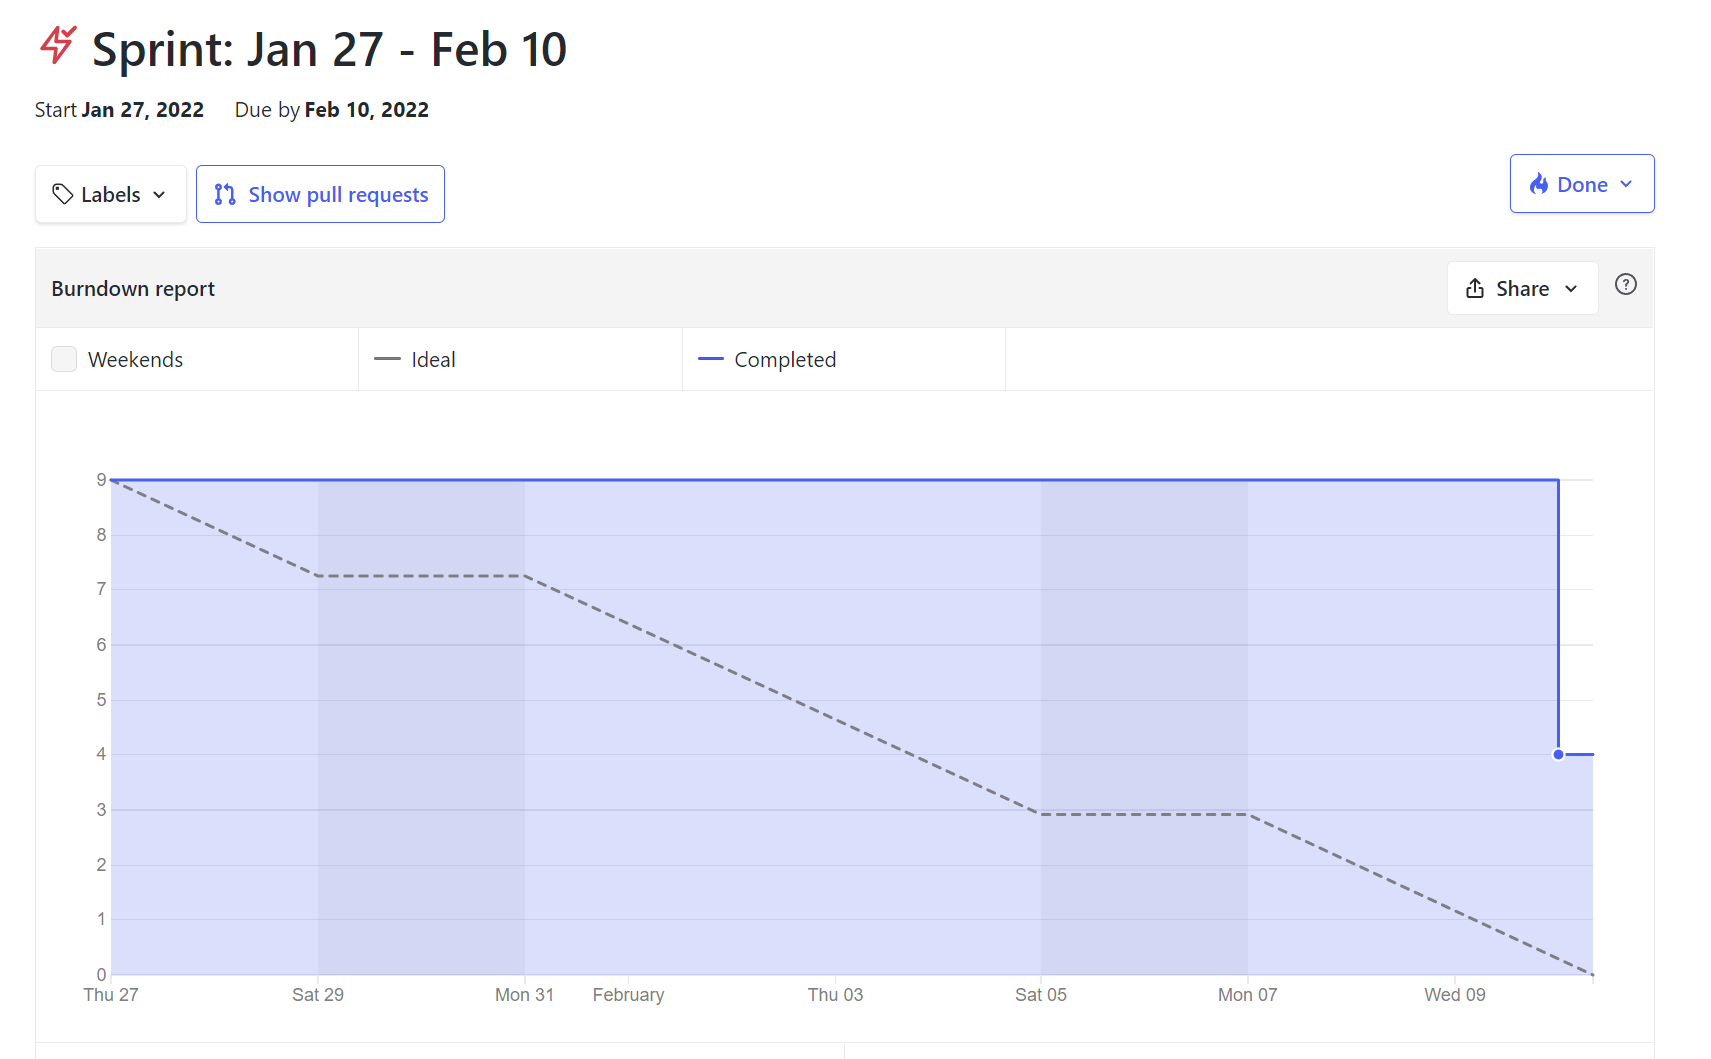
\includegraphics[width=1\textwidth]{AnexA_First_Memory_BurnDown}
	\caption{Primeras \textit{issues} relacionadas con la memoria}
	\label{fig:AnexA_First_Memory_BurnDown}
\end{figure}
\FloatBarrier

\subsubsection{Fase de implementación de mejoras y nueva funcionalidad}
La más larga de todas las fases con una duración de unos 7 \textit{sprints} (14 semanas). En esta fase se realizaron las tareas de desarrollo entre las que destacan:

\begin{itemize}
	\item Actualización del código previo y dependencias.
	\item Corrección de \textit{bugs}  existentes.
	\item Mejora del motor de cálculo de métricas para casos poco comunes.
	\item Mejoras de interfaz y usabilidad (leyenda, tooltips, separación por grupos de métricas, botones para cerrar diálogos, etc.)
	\item Nuevas métricas \textit{CICD}: IC1, IC2, IC3, P1 y P2
	\item Adaptación de las funcionalidades a las nuevas métricas (export, import, actualización, etc.)
	\item Integración con \textit{GitHub} y adaptación de la interfaz.
\end{itemize}

Las \textit{issues} que se han realizado en esta fase son:

\begin{figure}[!h]
	\centering
	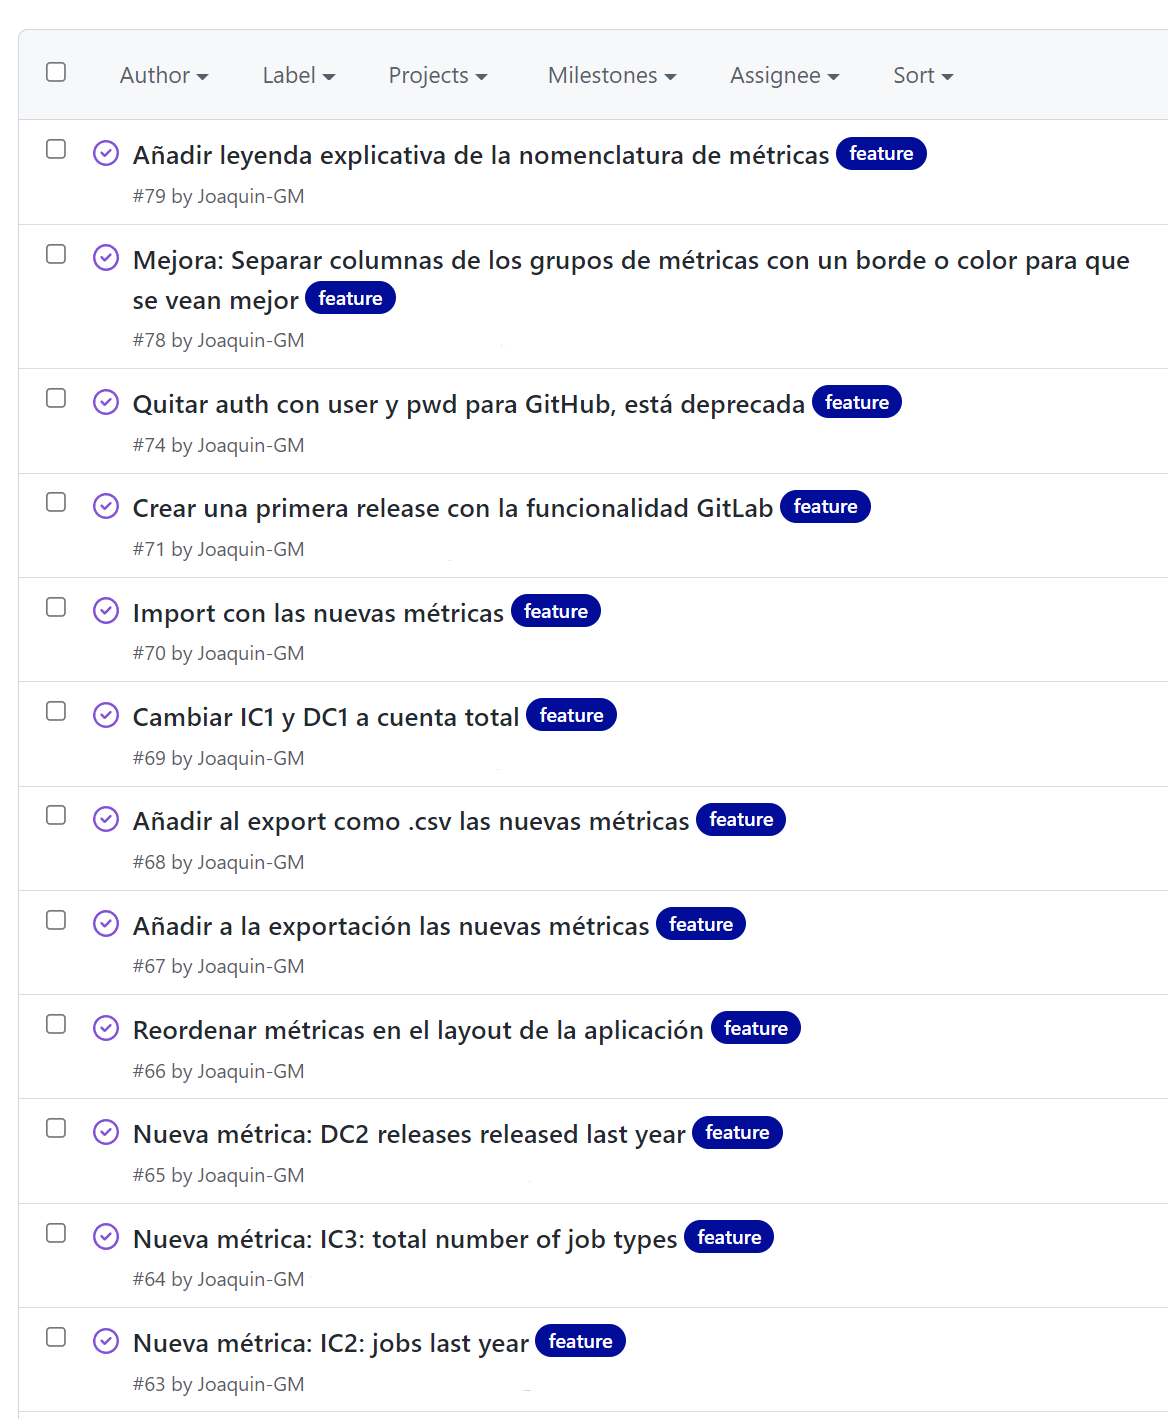
\includegraphics[width=1\textwidth]{AnexA_First_Develop_Issues}
	\caption{\textit{Issues} de desarrollo 1/2}
	\label{fig:AnexA_First_Develop_Issues}
\end{figure}
\FloatBarrier

\begin{figure}[!h]
	\centering
	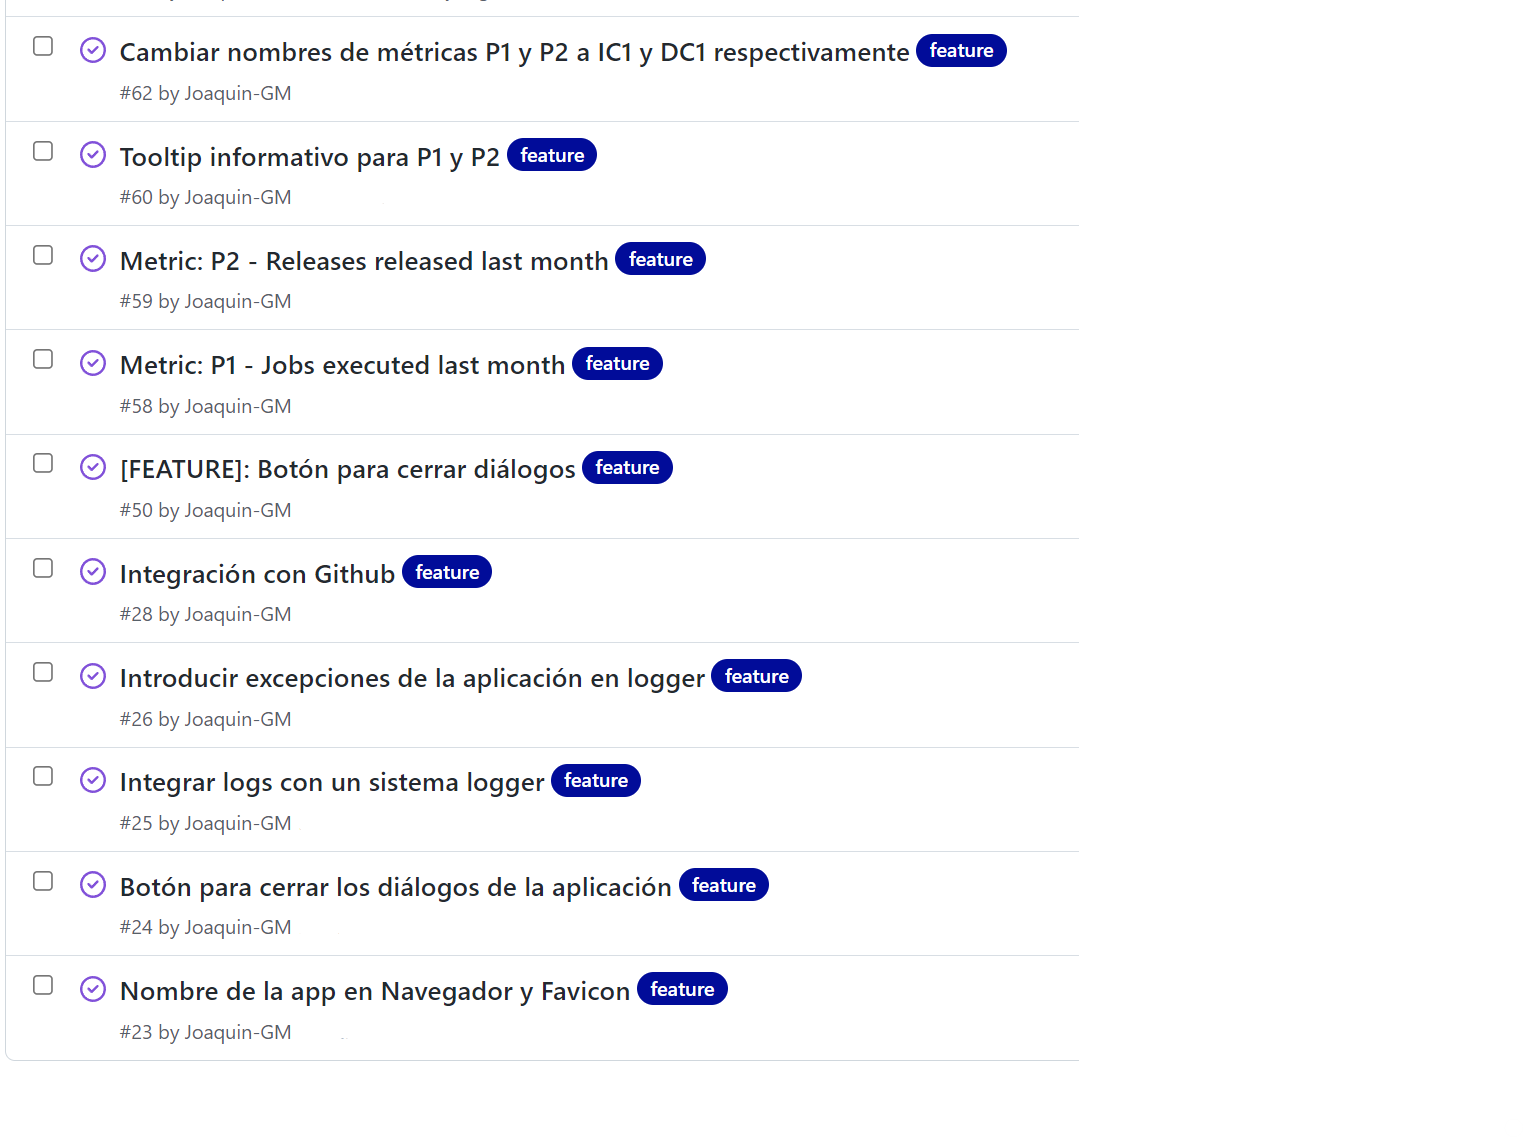
\includegraphics[width=1\textwidth]{AnexA_Second_Develop_Issues}
	\caption{\textit{Issues} de desarrollo 2/2}
	\label{fig:AnexA_Second_Develop_Issues}
\end{figure}
\FloatBarrier

Un ejemplo de gráfico \textit{burndown} de uno de los \textit{sprints} de esta fase puede verse en la figura \ref{fig:AnexA-Develop_BurnDown}

\begin{figure}[!h]
	\centering
	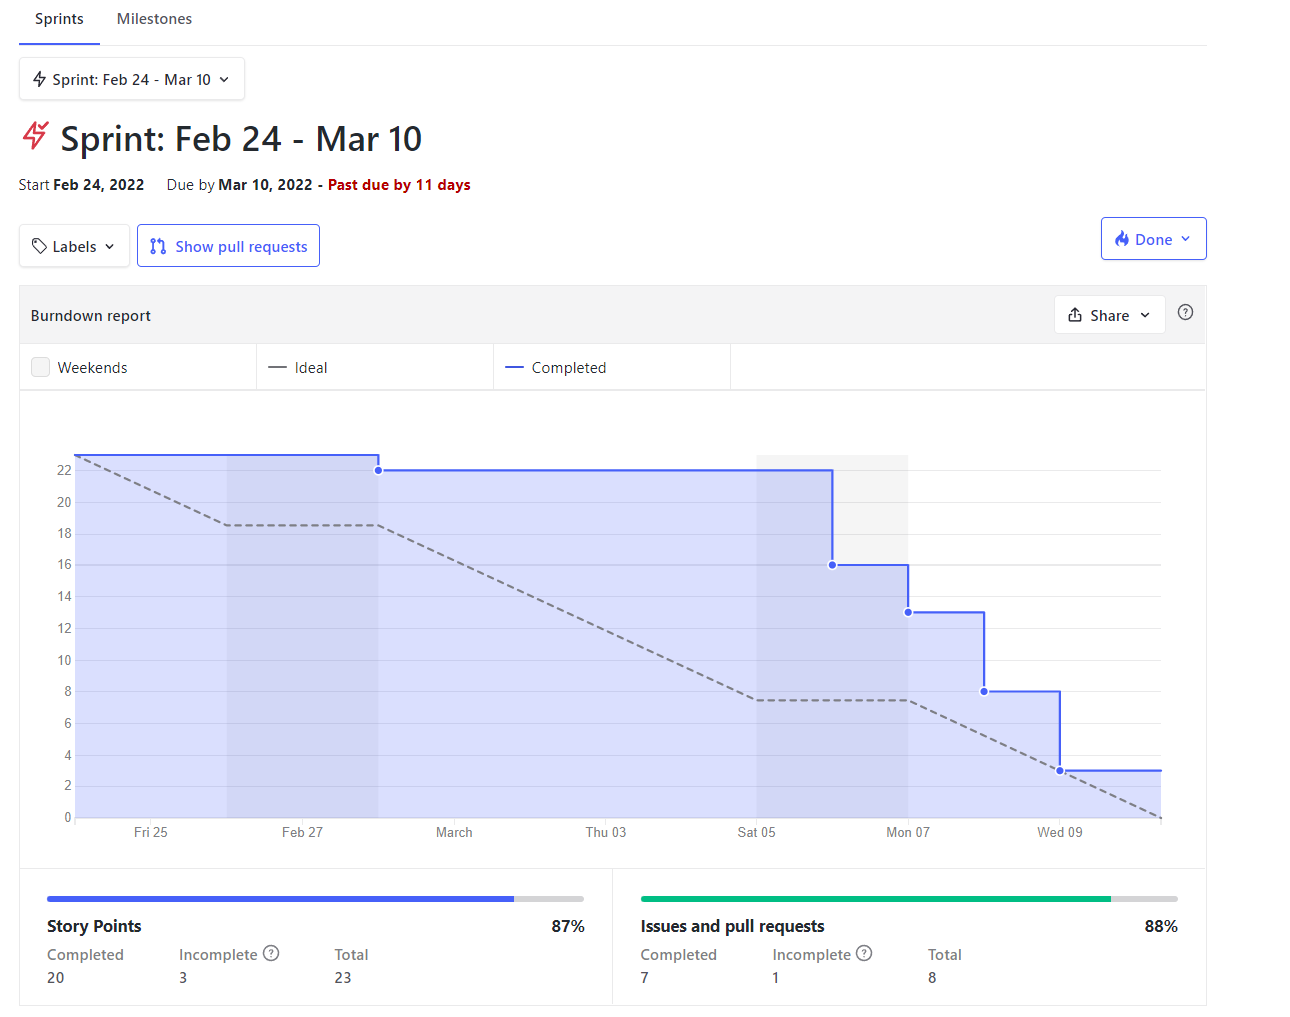
\includegraphics[width=1\textwidth]{AnexA-Develop_BurnDown}
	\caption{\textit{Burndown} de un \textit{sprint} de desarrollo}
	\label{fig:AnexA-Develop_BurnDown}
\end{figure}
\FloatBarrier

En este caso se puede observar que sí se completaron todas las \textit{issues} menos una. Se puede apreciar en el gráfico que durante los primeros días del \textit{sprint} no se pudo terminar ninguna \textit{issue}, si se hubiera podido conseguir nos habríamos aproximado más al avance ideal y probablemente se hubiera podido cerrar la \textit{issue} pendiente de ese sprint.

\subsubsection{Segunda fase de documentación}
En esta última fase de documentación se trabajó durante 2 \textit{sprint} (4 semanas) en los siguientes apartados:

\begin{itemize}
	\item Memoria: Aspectos relevantes del desarrollo del proyecto
	\item Memoria: Trabajos relacionados
	\item Memoria: Conclusiones y líneas de trabajo futuras
	\item Anexos
	\item Vídeos de presentación del proyecto
\end{itemize}

A continuación podemos ver las \textit{issues} con las que se trabajó en esta fase:

\begin{figure}[!h]
	\centering
	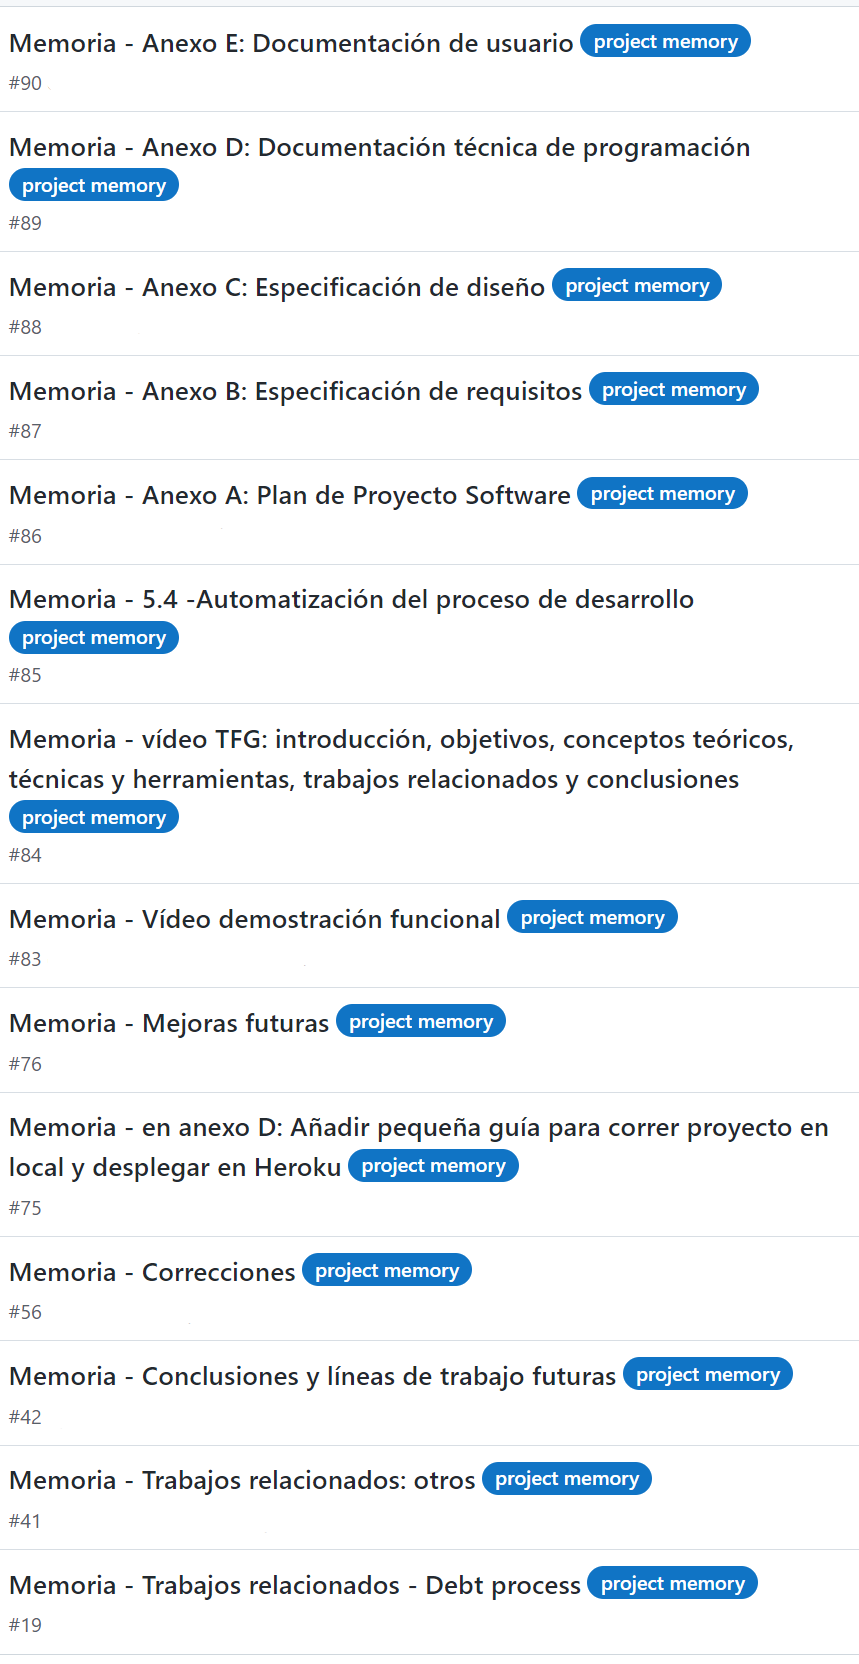
\includegraphics[width=0.7\textwidth]{AnexA_Second_Memory_Issues}
	\caption{Últimas \textit{issues} relacionadas con la memoria, anexos y documentación}
	\label{fig:AnexA_Second_Memory_Issues}
\end{figure}
\FloatBarrier

Un último ejemplo de gráfico \textit{burndown} de esta fase en el que sí se fue avanzando siguiendo el avance ideal:

\begin{figure}[!h]
	\centering
	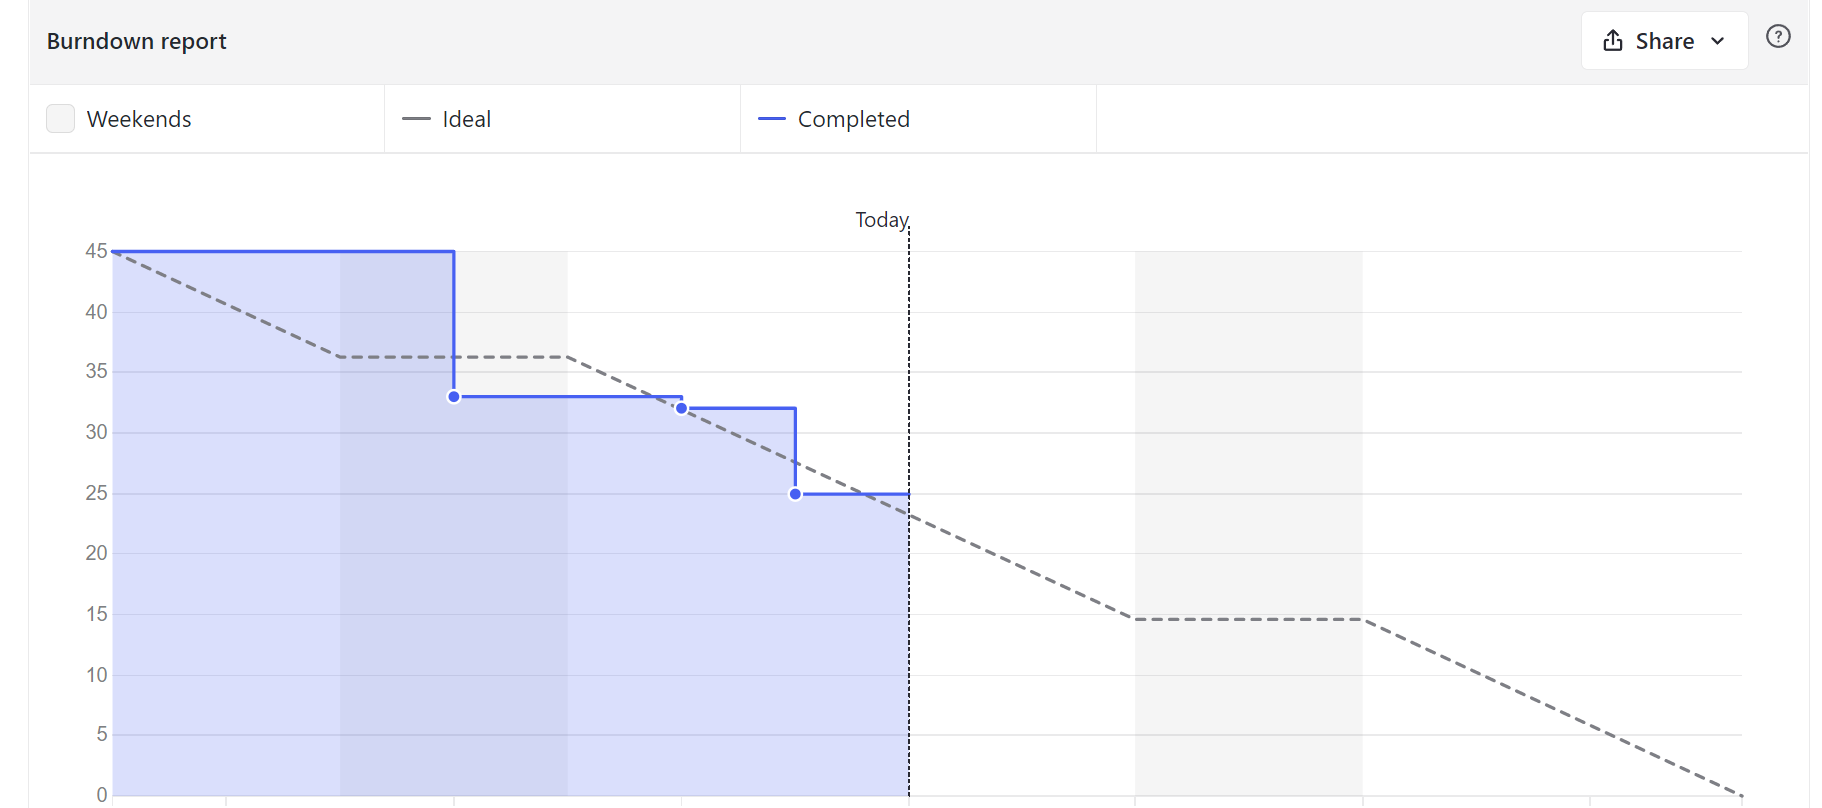
\includegraphics[width=1\textwidth]{AnexA-Second_Memory_BurnDown}
	\caption{\textit{Burndown} del último \textit{sprint} de documentación}
	\label{fig:AnexA-Second_Memory_BurnDown}
\end{figure}
\FloatBarrier


\section{Estudio de viabilidad}
\subsection{Viabilidad económica}
A continuación se va a realizar un estudio del coste que supondría haber realizado el proyecto en un entorno real y se analizan posibles maneras de monetizar el proyecto para cubrir este coste.

\subsubsection{Costes}
\textbf{Costes de personal}

Es el mayor de los costes como en prácticamente todos los proyectos de desarrollo de software, el proyecto ha sido realizado por una persona con una jornada reducida de unas 12 horas semanales (debido a la simultaneidad del desarrollo del proyecto con la actividad laboral del alumno) durante 8 meses (mediados de octubre 2021 hasta mediados de junio de 2022). Se pueden estimar los siguientes valores:
\begin{itemize}
	\tightlist
	\item Salario neto mensual: 500 \officialeuro
	\item Retención por IRPF de carácter general del 15\% \cite{agencia_tributaria_cuadro_2022}
	\item Una retribución a la Seguridad Social de 28,3\% \cite{ministerio_de_empleo_y_seguridad_social_bases_2022}: Empresa (23,6\%) +  Trabajador(Desempleo de tipo general + FOGASA + Formación profesional)(4,70\%)
\end{itemize}

Realizando cálculos, se obtiene:
\begin{longtable}[]{@{}lr@{}}
	\toprule
	\begin{minipage}[b]{0.38\columnwidth}\raggedright\strut
		\textbf{Concepto}\strut
	\end{minipage} & \begin{minipage}[b]{0.40\columnwidth}\raggedright\strut
		\textbf{Coste}\strut
	\end{minipage}\tabularnewline
	\midrule
	\endhead
	\begin{minipage}[t]{0.38\columnwidth}\raggedright\strut
		Salario mensual neto\strut
	\end{minipage} & \begin{minipage}[t]{0.40\columnwidth}\raggedright\strut
		500 \officialeuro (12h/semana)\strut
	\end{minipage}\tabularnewline
	\begin{minipage}[t]{0.38\columnwidth}\raggedright\strut
		Retención IRPF (15\%)\strut
	\end{minipage} & \begin{minipage}[t]{0.40\columnwidth}\raggedright\strut
		122,15 \officialeuro\strut
	\end{minipage}\tabularnewline
	\begin{minipage}[t]{0.38\columnwidth}\raggedright\strut
		Seguridad Social (29,9\%)\strut
	\end{minipage} & \begin{minipage}[t]{0.40\columnwidth}\raggedright\strut
		192,18 \officialeuro\strut
	\end{minipage}\tabularnewline
	\begin{minipage}[t]{0.38\columnwidth}\raggedright\strut
		Salario mensual bruto\strut
	\end{minipage} & \begin{minipage}[t]{0.40\columnwidth}\raggedright\strut
		814,33 \officialeuro\strut
	\end{minipage}\tabularnewline
	\midrule
	\begin{minipage}[t]{0.38\columnwidth}\raggedright\strut
		\textbf{Total 8 meses}\strut
	\end{minipage} & \begin{minipage}[t]{0.40\columnwidth}\raggedright\strut
		4.314,33 \officialeuro\strut
	\end{minipage}\tabularnewline
	\bottomrule
	\caption{Costes de personal}
\end{longtable}

\textbf{Costes de hardware}

Se va a considerar como coste únicamente un ordenador, hay que tener en cuenta que el período de amortización de equipos para procesos de información es de 8 años \cite{agencia_tributaria_tabla_2022}, que se considera un coste de 800 \officialeuro \thinspace para dicho ordenador y que se ha usado durante 8 meses:

\begin{longtable}[]{@{}lrr@{}}
	\toprule
	\begin{minipage}[b]{0.29\columnwidth}\raggedright\strut
		\textbf{Concepto}\strut
	\end{minipage} & \begin{minipage}[b]{0.18\columnwidth}\raggedright\strut
		\textbf{Coste}\strut
	\end{minipage} & \begin{minipage}[b]{0.32\columnwidth}\raggedright\strut
		\textbf{Coste amortizado}\strut
	\end{minipage}\tabularnewline
	\midrule
	\endhead
	\begin{minipage}[t]{0.29\columnwidth}\raggedright\strut
		Ordenador portátil\strut
	\end{minipage} & \begin{minipage}[t]{0.18\columnwidth}\raggedright\strut
		800 \officialeuro\strut
	\end{minipage} & \begin{minipage}[t]{0.32\columnwidth}\raggedright\strut
		66,67 \officialeuro\strut
	\end{minipage}\tabularnewline
	\midrule
	\begin{minipage}[t]{0.29\columnwidth}\raggedright\strut
		\textbf{Total}\strut
	\end{minipage} & \begin{minipage}[t]{0.18\columnwidth}\raggedright\strut
		800 \officialeuro\strut
	\end{minipage} & \begin{minipage}[t]{0.32\columnwidth}\raggedright\strut
		66,67 \officialeuro\strut
	\end{minipage}\tabularnewline
	\bottomrule
	\caption{Costes de hardware}
\end{longtable}

\textbf{Costes de software}

Todo el software empleado para el desarrollo del proyecto tiene licencias gratuitas, salvo el propio sistema operativo. Se ha utilizado \textit{Windows 11} en este caso y se ha trabajado con una licencia que tiene un coste muy reducido de unos 12 \officialeuro al ser una clave \textit{OEM} (que son perfectamente legales).\\
Teniendo en cuenta dicho coste y que la amortización para sistemas y programas informáticos es de 6 años \cite{agencia_tributaria_tabla_2022} y se ha utilizado durante 8 meses:

\begin{longtable}[]{@{}lrr@{}}
	\toprule
	\begin{minipage}[b]{0.29\columnwidth}\raggedright\strut
		\textbf{Concepto}\strut
	\end{minipage} & \begin{minipage}[b]{0.18\columnwidth}\raggedright\strut
		\textbf{Coste}\strut
	\end{minipage} & \begin{minipage}[b]{0.32\columnwidth}\raggedright\strut
		\textbf{Coste amortizado}\strut
	\end{minipage}\tabularnewline
	\midrule
	\endhead
	\begin{minipage}[t]{0.29\columnwidth}\raggedright\strut
		\textit{Windows 10 Home}\strut
	\end{minipage} & \begin{minipage}[t]{0.18\columnwidth}\raggedright\strut
		12 \officialeuro\strut
	\end{minipage} & \begin{minipage}[t]{0.32\columnwidth}\raggedright\strut
		1,33 \officialeuro\strut
	\end{minipage}\tabularnewline
	\midrule
	\begin{minipage}[t]{0.29\columnwidth}\raggedright\strut
		\textbf{Total}\strut
	\end{minipage} & \begin{minipage}[t]{0.18\columnwidth}\raggedright\strut
		12 \officialeuro\strut
	\end{minipage} & \begin{minipage}[t]{0.32\columnwidth}\raggedright\strut
		1,33 \officialeuro\strut
	\end{minipage}\tabularnewline
	\bottomrule
	\caption{Costes de software}
\end{longtable}

\textbf{Otros costes}
Se van a tener en cuenta además otros costes necesarios para poder desarrollar el proyecto en un entorno real. Se va a considerar una opción algo pesimista en la que es necesario alquilar una oficina para el desarrollador con sus costes asociados durante los 8 meses de desarrollo (alquiler unos 50 \officialeuro al mes, internet unos 30 \officialeuro al mes y algo de material de oficina):\\

\begin{longtable}[]{@{}lr@{}}
	\toprule
	\begin{minipage}[b]{0.48\columnwidth}\raggedright\strut
		\textbf{Concepto}\strut
	\end{minipage} & \begin{minipage}[b]{0.18\columnwidth}\raggedright\strut
		\textbf{Coste}\strut
	\end{minipage}\tabularnewline
	\midrule
	\endhead
	\begin{minipage}[t]{0.48\columnwidth}\raggedright\strut
		Alquiler de oficina\strut
	\end{minipage} & \begin{minipage}[t]{0.18\columnwidth}\raggedright\strut
		400 \officialeuro\strut
	\end{minipage}\tabularnewline
	\begin{minipage}[t]{0.48\columnwidth}\raggedright\strut
		Internet\strut
	\end{minipage} & \begin{minipage}[t]{0.18\columnwidth}\raggedright\strut
		240 \officialeuro\strut
	\end{minipage}\tabularnewline
	\begin{minipage}[t]{0.48\columnwidth}\raggedright\strut
		Material de oficina\strut
	\end{minipage} & \begin{minipage}[t]{0.18\columnwidth}\raggedright\strut
		40 \officialeuro\strut
	\end{minipage}\tabularnewline
	\midrule
	\begin{minipage}[t]{0.48\columnwidth}\raggedright\strut
		\textbf{Total}\strut
	\end{minipage} & \begin{minipage}[t]{0.18\columnwidth}\raggedright\strut
		680 \officialeuro\strut
	\end{minipage}\tabularnewline
	\bottomrule
	\caption{Costes varios.}
\end{longtable}

\textbf{Coste total}

El coste total por tanto sería:\\

\begin{longtable}[]{@{}lr@{}}
	\toprule
	\begin{minipage}[b]{0.22\columnwidth}\raggedright\strut
		\textbf{Concepto}\strut
	\end{minipage} & \begin{minipage}[b]{0.22\columnwidth}\raggedright\strut
		\textbf{Coste}\strut
	\end{minipage}\tabularnewline
	\midrule
	\endhead
	\begin{minipage}[t]{0.22\columnwidth}\raggedright\strut
		Personal\strut
	\end{minipage} & \begin{minipage}[t]{0.22\columnwidth}\raggedright\strut
		4.314,33 \officialeuro\strut
	\end{minipage}\tabularnewline
	\begin{minipage}[t]{0.22\columnwidth}\raggedright\strut
		Hardware\strut
	\end{minipage} & \begin{minipage}[t]{0.22\columnwidth}\raggedright\strut
		66,67 \officialeuro\strut
	\end{minipage}\tabularnewline
	\begin{minipage}[t]{0.22\columnwidth}\raggedright\strut
		Software\strut
	\end{minipage} & \begin{minipage}[t]{0.22\columnwidth}\raggedright\strut
		1,33 \officialeuro\strut
	\end{minipage}\tabularnewline
	\begin{minipage}[t]{0.22\columnwidth}\raggedright\strut
		Otros\strut
	\end{minipage} & \begin{minipage}[t]{0.22\columnwidth}\raggedright\strut
		680 \officialeuro\strut
	\end{minipage}\tabularnewline
	\midrule
	\begin{minipage}[t]{0.22\columnwidth}\raggedright\strut
		Total\strut
	\end{minipage} & \begin{minipage}[t]{0.22\columnwidth}\raggedright\strut
		5.062,33 \officialeuro\strut
	\end{minipage}\tabularnewline
	\bottomrule
	\caption{Costes totales.}
\end{longtable}

\subsubsection{Beneficios}

Actualmente la aplicación tiene licencia libre y es gratuita por lo que no se obtiene ningún beneficio con ella. Para poder obtenerlos se pueden plantear diferentes alternativas:

\begin{itemize}
	\item Pago a través de licencias de uso.
	\item Pago por subscripción al servicio.
	\item Incluir publicidad, esta solución podría ser la mejor si queremos cubrir costes y que el proyecto siga siendo de uso gratuito.
\end{itemize}


\subsection{Viabilidad legal}
Nuestro software al trabajar con repositorios públicos o aquellos a los que el usuario tenga acceso no puede incumplir con la privacidad de los mismos, por tanto, lo que hay que analizar son las licencias del software que se ha usado durante desarrollo de la aplicación.\\
 En la Fig. \ref{fig:AnexA_Licencias} podemos ver los artefactos utilizados en el proyecto (dependencias del proyecto en el fichero \ruta{pom.xml}:) y cuya información se puede obtener en el repositorio de \textit{Maven} \footnote{\url{https://mvnrepository.com/}} 

\begin{figure}[!h]
	\centering
	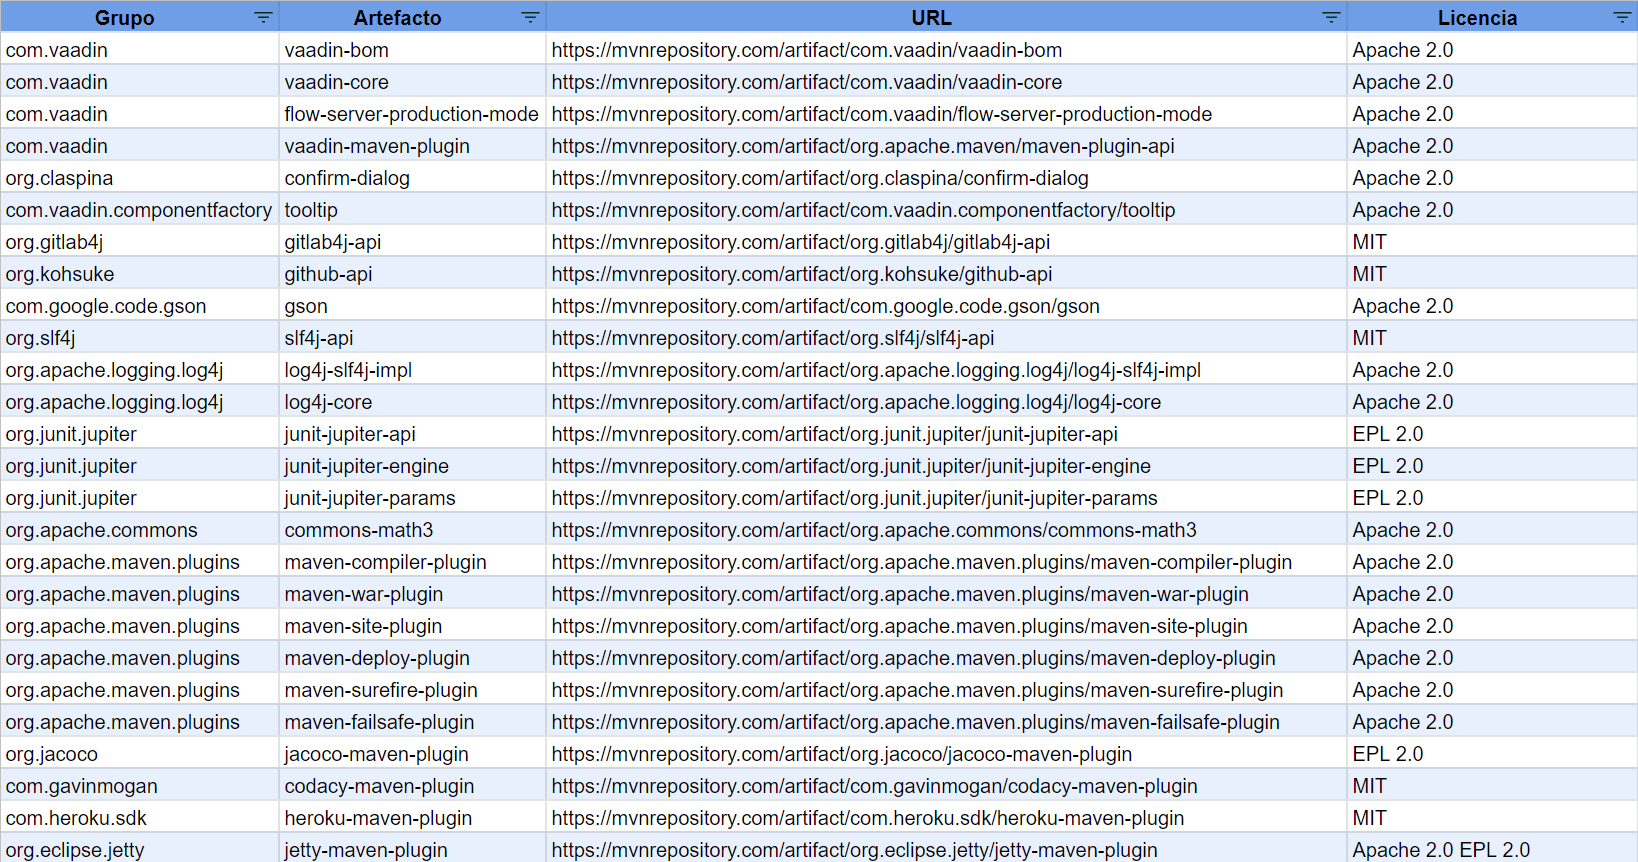
\includegraphics[scale=0.32]{AnexA_Licencias}
	\caption{Licencias de las dependencias del proyecto}
	\label{fig:AnexA_Licencias}
\end{figure}
\FloatBarrier

Por lo tanto, las licencias a las que está sometido nuestro proyecto son, de más a menos permisivas:
\begin{itemize}
	\item \textit{MIT}
	\item \textit{Apache v.2.0}
	\item \textit{EPL 2.0}
\end{itemize}

La licencia más restrictiva de las tres es la \textit{Eclipse Public License} que es la que tienen las librerías que se utilizan para pruebas (JUnit).

A este proyecto se le podría dar la licencia \textit{GNU General Public License v3.0}, que permite el uso comercial, modificación, distribución, uso privado y el uso de patentes mientas queramos que siga siendo de acceso y uso público como hasta ahora.
Esta licencia es compatible con las del software utilizado en el proyecto pues la versión \textit{EPL 2.0} permite utilizar la versión 2 de la \textit{GPL} de \textit{GNU} y posteriores como licencia secundaria en una parte específica del código. Por esto, se garantiza la compatibilidad de ese código con esas versiones de la GPL \cite{santiago_lista_2019}.

\apendice{Especificación de Requisitos}\label{anex:B}

\section{Introducción}

En este anexo se analizan y documentan las diferentes necesidades funcionales y no funcionales que deberán ser soportadas por la aplicación generada en este proyecto. Se van a nombrar tanto los requisitos del proyecto original\cite{TFGPrevio} como los del proyecto actual pues éste último ha de cumplir ambos.


\section{Objetivos generales}
El objetivo general de este TFG es mantener la funcionalidad implementada en el proyecto original\cite{TFGPrevio} y mejorarla incluyendo nuevas métricas y realizando la integración con \textit{GitHub}para poder trabajar con repositorios alojados allí. Además se implementarán mejoras de la interfaz para mejorar la usabilidad y se corregirán errores.

Por tanto se pueden nombrar los siguientes objetivos:
\begin{itemize}
	\tightlist
	\item Se obtendrán medidas de métricas de evolución de uno o varios proyectos alojados en repositorios tanto en \textit{GitLab} como en \textit{GitHub}.
	\item Las métricas que se desean calcular de un repositorio  son algunas de las especificadas en la tesis titulada ``\textit{sPACE: Software Project Assessment in the Course of Evolution}'' \cite{ratzinger_space:_2007} y 
	adaptadas a los repositorios software junto a nuevas métricas relacionadas con la integración y despliegue continuos (las 5 últimas):
	\begin{itemize}
		\tightlist
		\item Número total de incidencias (\textit{issues})
		\item Cambios (\textit{commits}) por incidencia
		\item Porcentaje de incidencias cerrados
		\item Media de días en cerrar una incidencia
		\item Media de días entre cambios
		\item Días entre primer y último cambio
		\item Rango de actividad de cambios por mes
		\item Porcentaje de pico de cambios
		\item Número total de \textit{jobs} ejecutados
		\item Número de \textit{jobs} ejecutados el último año
		\item Número de tipos diferentes de \textit{jobs} ejecutados
		\item Número total de \textit{releases}
		\item Número de \textit{releases} lanzadas el último año
		
	\end{itemize}
	\item Se pretende ser capaces de evaluar el estado de un proyecto comparándolo con otros proyectos por medio del uso de las métricas anteriores. Para ello se deberán establecer unos valores umbrales por cada métrica basados en el cálculo de los cuartiles Q1 y Q3.\\
	 Además, estos valores se podrán calcular dinámicamente y se almacenarán en perfiles de configuración de métricas. Estos umbrales deberán existir para todas la métricas, incluidas las nuevas.
	\item Se dará la posibilidad de almacenar de manera persistente estos perfiles de métricas para permitir comparaciones futuras. 
	\item También se permitirá almacenar de forma persistente las métricas obtenidas de los repositorios para su posterior consulta o tratamiento. Esto permitiría comparar nuevos proyectos con proyectos de los que ya se han calculado sus métricas.
	\item La persistencia debe incluir también las nuevas métricas, tanto para la exportación como para la importación de los valores de las mismas.
\end{itemize}

\section{Objetivos técnicos}
Este apartado resume requisitos del proyecto más técnicos y centrados en el proceso y otras características no funcionales.
\begin{itemize}
	\tightlist
	\item Utilizar el diseño basado en \textit{frameworks}  y en patrones de diseño \cite{gamma_patrones_2002} existente para implementar las nuevas métricas.
	\item Utilizar y adaptar en lo necesario el diseño de la aplicación para extender a \textit{GitHub}su funcionalidad y seguir permitiendo la extensión otras plataformas de desarrollo colaborativo como \textit{Bitbucket}.
	\item Crear una batería de pruebas automáticas en los subsistemas de lógica de la aplicación.
	\item Utilizar una plataforma de desarrollo colaborativo que incluya un sistema de control de versiones, un sistema de seguimiento de incidencias y que permita una comunicación fluida entre el tutor y el alumno. Se sugiere la utilización de \textit{GitHub}.
	\item Utilizar un sistema de integración y despliegue continuo.
	\item Mejorar la gestión de errores existente tratando excepciones de biblioteca y de la propia aplicación y registrar dichos eventos de error e información en ficheros de \textit{log}. 
	\item Probar la aplicación con ejemplos reales y utilizando técnicas avanzadas, como entrada de datos de test en ficheros con formato tabulado tipo CSV (\textit{Comma Separated Values}). 	
\end{itemize}

\section{Actores}
Se consideran dos actores:
\begin{itemize}
	\tightlist
	\item El usuario de la aplicación, es aquella persona que utilice la aplicación.
	\item El desarrollador, que a su vez puede ser considerado como usuario pero que además tiene las labores de implementación y mantenimiento de la aplicación.
\end{itemize}

\section{Catálogo de requisitos}
En esta sección se van a enumerar los requisitos que el sistema tendrá que satisfacer. Están divididos en dos tipos, en el primero se basa en funcionalidad y el segundo en aspectos del proceso de desarrollo y aspectos técnicos del sistema como la mantenibilidad.

\subsection{Requisitos funcionales}

\begin{itemize}
\item \textbf{RF-1} Establecer conexión con \textit{GitHub}: El usuario debe poder establecer conexión con \textit{GitHub}.
	\begin{itemize}
		\item \textbf{RF-1.1} Debido a las restriccones que tiene la \textit{API} de \textit{GitHub} y que se \textit{deprecó} el acceso del usuario por usuario y contraseña\footnote{Autenticación en \textit{GitHub API} - \url{https://docs.github.com/es/rest/overview/other-authentication-methods}}, el usuario podrá iniciar sesión desde la aplicación sólo mediante un token de acceso personal a su usuario en \textit{GitHub}para poder obtener los repositorios públicos y privados a los que tenga acceso.
		\item \textbf{RF-1.2} La aplicación mostrará al usuario en todo momento la conexión que está utilizando
		\item \textbf{RF-1.3} El usuario podrá utilizar la aplicación sin establecer una conexión. Aunque no tenga acceso a los repositorios de \textit{GitHub}.
		\item \textbf{RF-1.4} El usuario podrá cambiar de conexión teniendo en cuenta que solo puede haber un tipo de conexión con \textit{GitHub} activo en un instante dado. Esta conexión será independiente de la posible conexión con \textit{GitLab}.

	\end{itemize}
	\item \textbf{RF-2} Establecer conexión con \textit{GitLab}: El usuario debe poder establecer distintos tipos de conexión a \textit{GitLab}.
	\begin{itemize}
		\item \textbf{RF-2.1} El usuario podrá iniciar sesión desde la aplicación mediante usuario y contraseña a su usuario en \textit{GitLab} para poder obtener los repositorios públicos y privados a los que tenga acceso.
		\item \textbf{RF-2.2} El usuario podrá iniciar sesión desde la aplicación mediante un token de acceso personal a su usuario en \textit{GitLab} para poder obtener los repositorios públicos y privados a los que tenga acceso.
		\item \textbf{RF-2.3} El usuario podrá establecer una conexión pública a \textit{GitLab} para poder obtener los repositorios públicos.
		\item \textbf{RF-2.4} El usuario podrá utilizar la aplicación sin establecer una conexión. Aunque no tenga acceso a los repositorios de \textit{GitLab}.
		\item \textbf{RF-2.5} El usuario deberá elegir un tipo de conexión al entrar por primera vez a la aplicación.
		\item \textbf{RF-2.6} La aplicación mostrará al usuario en todo momento la conexión que está utilizando
		\item \textbf{RF-2.7} El usuario podrá cambiar de conexión teniendo en cuenta que solo puede haber un tipo de conexión con \textit{GitLab} activo en un instante dado. Esta conexión será independiente de la posible conexión con \textit{GitHub}.
	\end{itemize}
	\item \textbf{RF-3} Gestión de proyectos. El usuario podrá calcular las métricas de proyectos tanto de \textit{GitHub}como de \textit{GitLab} definidas en la sección \ref{sect:B_5_1_1}: `\textit{Definición de las métricas}' y se mostrarán los resultados en forma de tabla en la que las filas se correspondan con los proyectos y las columnas con las métricas.
	\begin{itemize}
		\item \textbf{RF-3.1} El usuario podrá añadir un proyecto siempre que tenga una conexión a \textit{GitLab} o con \textit{GitHub}(dependiendo del dónde esté alojado dicho proyecto):
		\begin{itemize}
			\item \textbf{RF-3.1.1} El usuario podrá añadir un proyecto a partir del nombre de usuario o ID del propietario y el nombre del proyecto, siempre que tenga acceso desde la conexión establecida.
			\item \textbf{RF-3.1.2} El usuario podrá añadir un proyecto a partir del nombre o del ID del grupo al que pertenece el proyecto y su nombre, siempre que tenga acceso desde la conexión establecida.
			\item \textbf{RF-3.1.3} El usuario podrá añadir un proyecto a partir de su URL, siempre que tenga acceso desde la conexión establecida.
		\end{itemize}
		\item \textbf{RF-3.2} El usuario no podrá añadir un proyecto que ya esté en la tabla.
		\item \textbf{RF-3.3} Al añadir un proyecto a la tabla se calcularán las métricas definidas en la sección \ref{sect:B_5_1_1}: `\textit{Definición de las métricas}' y se mostrarán en forma de tabla.
		\item \textbf{RF-3.4} El usuario podrá eliminar un proyecto de la tabla.
		\item \textbf{RF-3.5} El usuario podrá volver a obtener las métricas de un repositorio que ya haya añadido, siempre que tenga acceso desde la conexión establecida (con \textit{GitHub}o \textit{GitLab} dependiendo de dónde esté alojado el proyecto).
		\item \textbf{RF-3.6} El usuario podrá exportar los proyectos y sus métricas a un fichero con formato `\ruta{.emr}'.
		\item \textbf{RF-3.7} El usuario podrá exportar los resultados de las métricas de todos los proyectos en un fichero con formato CSV.
		\item \textbf{RF-3.8} El usuario podrá importar y añadir repositorios a la tabla  desde un fichero con formato `\ruta{.emr}', respetando el requisito RF3.2 de no añadir un repositorio ya existente.
		\item \textbf{RF-3.9} El usuario podrá importar repositorios a la tabla, sobrescribiendo los de la tabla.
		\item \textbf{RF-3.10} Se podrán filtrar los proyectos por su nombre.
		\item \textbf{RF-3.11} Se puede ordenar los repositorios por nombre, fecha de medición y por cualquiera de las métricas.
		\item \textbf{RF-3.12} Al ordenar por las nuevas métricas relacionadas con \textit{CICD} habrá que tener en cuenta que habrá medidas que no se habrán calculado por falta de datos de \textit{GitLab} si no se ha realizado conexión \textit{autenticada} pues \textit{GitLab API} no devuelve información  sobre \textit{jobs} y \textit{releases} con conexión pública.
	\end{itemize}
	\item \textbf{RF-4} Evaluación de métricas. Las métricas, una vez calculadas, serán evaluadas mediante un código de color (verde - bueno, naranja - peligro, rojo - malo) a partir de un perfil de métricas, que será un conjunto de valores mínimo y máximo de cada una de las métricas, a partir de la definición de la evaluación en la sección \ref{sect:B_5_1_2}: `\textit{Evaluación de métricas}'. Esto ha de aplicar también a las nuevas métricas que se implementen no sólo a las existentes.
	\begin{itemize}
		\item \textbf{RF-4.1} Se podrá cargar un perfil de métricas que contenga valores umbrales mínimo y máximo y se utilizarán para evaluarlas.
		\item \textbf{RF-4.2} El usuario podrá cargar un perfil por defecto creado a partir de un conjunto de datos \footnote{\url{https://github.com/clopezno/clopezno.github.io/blob/master/agile_practices_experiment/DataSet_EvolutionSoftwareMetrics_FYP.csv}} de un estudio empírico de las métricas de evolución del software en trabajos finales de grado\cite{lopez_nozal_measuring_2019}.
		\item \textbf{RF-4.3} El usuario podrá cargar un perfil creado a partir de los repositorios que existan en la tabla.
		\item \textbf{RF-4.4} El usuario podrá exportar el perfil de métricas que tenga cargado a un fichero con formato \ruta{emmp}.
		\item \textbf{RF-4.5} El usuario podrá importar un perfil de métricas que haya guardado anteriormente para evaluar los repositorios que tenga en la tabla.
		\item \textbf{RF-4.6} En un instante, solo puede haber un perfil de métricas cargado.
		\item \textbf{RF-4.7} Al inicio se cargará el perfil de evaluación por defecto.
	\end{itemize}
\end{itemize}

\subsubsection{Definición de las métricas}\label{sect:B_5_1_1}

En el requisito RF-3 implica que se deben calcular las siguientes métricas de un proyecto:

\textbf{\underline{I1 - Número total de \textit{issues} (incidencias)}}

\begin{itemize}
	\item \textbf{Categoría}: Proceso de Orientación
	\item \textbf{Descripción}: Número total de \textit{issues} creadas en el repositorio
	\item \textbf{Propósito}: ¿Cuántas \textit{issues} se han definido en el repositorio?
	\item \textbf{Fórmula}: $NTI$. \textit{NTI = número total de \textit{issues}}
	\item \textbf{Fuente de medición}: Proyecto en una plataforma de desarrollo colaborativo.
	\item \textbf{Interpretación}: $NTI \geq 0$. Valores bajos indican que no se utiliza un sistema de seguimiento de incidencias, podría ser porque el proyecto acaba de comenzar
	\item \textbf{Tipo de escala}: Absoluta
	\item \textbf{Tipo de medida}: \textit{NTI = Contador}
\end{itemize}

\textbf{\underline{I2 - \textit{Commits} (cambios) por \textit{issue}}}

\begin{itemize}
	\item \textbf{Categoría}: Proceso de Orientación
	\item \textbf{Descripción}: Número de \textit{commits} por \textit{issue}
	\item \textbf{Propósito}: ¿Cuál es el volumen medio de trabajo de las \textit{issues}?
	\item \textbf{Fórmula}: $CI = \frac{NTC}{NTI}$. \textit{CI = Cambios por \textit{issue}, NTC = Número total de \textit{commits}, NTI = \textbf{Número} total de \textit{issues}}
	\item \textbf{Fuente de medición}: Proyecto en una plataforma de desarrollo colaborativo.
	\item \textbf{Interpretación}: $CI \geq 1$, Lo normal son valores altos. Si el valor es menor que uno significa que hay desarrollo sin documentar.
	\item \textbf{Tipo de escala}: Ratio 
	\item \textbf{Tipo de medida}: \textit{NTC, NTI = Contador}
\end{itemize}

\textbf{\underline{I3 - Porcentaje de \textit{issues} cerradas}}

\begin{itemize}
	\item \textbf{Categoría}: Proceso de Orientación
	\item \textbf{Descripción}: Porcentaje de \textit{issues} cerradas
	\item \textbf{Propósito}: ¿Qué porcentaje de \textit{issues} definidas en el repositorio se han cerrado?
	\item \textbf{Fórmula}: $PIC = \frac{NTIC}{NTI}*100$. \textit{PIC = Porcentaje de \textit{issues} cerradas, NTIC = Número total de \textit{issues} cerradas, NTI = Número total de \textit{issues}}
	\item \textbf{Fuente de medición}: Proyecto en una plataforma de desarrollo colaborativo.
	\item \textbf{Interpretación}: $0 \leq PIC \leq 100$. Cuanto más alto mejor
	\item \textbf{Tipo de escala}: Ratio
	\item \textbf{Tipo de medida}: \textit{NTI, NTIC = Contador}
\end{itemize}

\textbf{\underline{TI1 - Media de días en cerrar una \textit{issue}}}

\begin{itemize}
	\item \textbf{Categoría}: Constantes de tiempo
	\item \textbf{Descripción}:  Media de días en cerrar una \textit{issue}
	\item \textbf{Propósito}: ¿Cuánto se suele tardar en cerrar una \textit{issue}? 
	\item \textbf{Fórmula}: $MDCI = \frac{\sum_{i=0}^{NTIC}DCI_i}{NTIC}$. \textit{MDCI = Media de días en cerrar una \textit{issue}, NTIC = Número total de \textit{issues} cerradas, DCI = Días en cerrar la \textit{issue}}
	\item \textbf{Fuente de medición}: Proyecto en una plataforma de desarrollo colaborativo.
	\item \textbf{Interpretación}: $MDCI \geq 0$. Cuanto más pequeño mejor. Si se siguen metodologías ágiles de desarrollo iterativo e incremental como \textit{SCRUM}, la métrica debería indicar la duración del \textit{sprint} definido en la fase de planificación del proyecto. En \textit{SCRUM} se recomiendan duraciones del \textit{sprint} de entre una y seis semanas, siendo recomendable que no exceda de un mes \cite{scrum_master_scrum_2019}.
	\item \textbf{Tipo de escala}: Ratio
	\item \textbf{Tipo de medida}: \textit{NTI, NTIC = Contador}
\end{itemize}

\textbf{\underline{TC1 - Media de días entre \textit{commits}}}

\begin{itemize}
	\item \textbf{Categoría}: Constantes de tiempo
	\item \textbf{Descripción}: Media de días que pasan entre dos \textit{commits} consecutivos
	\item \textbf{Propósito}: ¿Cuántos días suelen pasar desde un \textit{commit} hasta el siguiente?
	\item \textbf{Fórmula}: $MDC = \frac{\sum_{i=1}^{NTC} TC_i - TC_{i-1}}{NTC}$. $TC_i - TC_{i-1}$ en días; \textit{MDC = Media de días entre cambios, NTC = Número total de \textit{commits}, TC = Tiempo de \textit{commit}}
	%$MDEC = [Sumatorio de (TCi-TCj) desde i=1, j=0 hasta i=NTC] / NTC. NTC = Número total de \textit{commits}, TC = Tiempo de Commit$ 
	\item \textbf{Fuente de medición}: Proyecto en una plataforma de desarrollo colaborativo.
	\item \textbf{Interpretación}: $MDEC \geq 0$. Cuanto más pequeño mejor. Se recomienda no superar los 5 días.
	\item \textbf{Tipo de escala}: Ratio
	\item \textbf{Tipo de medida}: \textit{NTC = Contador; TC = Tiempo}
\end{itemize}

\textbf{\underline{TC2 - Días entre primer y último \textit{commit}}}

\begin{itemize}
	\item \textbf{Categoría}: Constantes de tiempo
	\item \textbf{Descripción}: Días transcurridos entre el primer y el ultimo \textit{commit} 
	\item \textbf{Propósito}: ¿Cuántos días han pasado entre el primer y el último \textit{commit}?
	\item \textbf{Fórmula}: $DEPUC = TC2- TC1$. $TC2- TC1$ en días;  \textit{DEPUC = Días entre primer y último \textit{commit}, TC2 = Tiempo de último \textit{commit}, TC1 = Tiempo de primer \textit{commit}}
	\item \textbf{Fuente de medición}: Proyecto en una plataforma de desarrollo colaborativo.
	\item \textbf{Interpretación}: $DEPUC \geq 0$. Cuanto más alto, más tiempo lleva en desarrollo el proyecto. En procesos software empresariales se debería comparar con la estimación temporal de la fase de planificación. 
	\item \textbf{Tipo de escala}: Absoluta
	\item \textbf{Tipo de medida}: \textit{TC = Tiempo}
\end{itemize}

\textbf{\underline{TC3 - Ratio de actividad de \textit{commits} por mes}}

\begin{itemize}
	\item \textbf{Categoría}: Constantes de tiempo
	\item \textbf{Descripción}: Muestra el número de \textit{commits} relativos al número de meses
	\item \textbf{Propósito}:¿Cuál es el número medio de cambios por mes?
	\item \textbf{Fórmula}: $RCM = \frac{NTC}{NM}$. \textit{RCM = Ratio de cambios por mes, NTC = Número total de \textit{commits}, NM = Número de meses que han pasado durante el desarrollo de la aplicación}
	\item \textbf{Fuente de medición}: Proyecto en una plataforma de desarrollo colaborativo.
	\item \textbf{Interpretación}: $RCM > 0$. Cuanto más alto mejor
	\item \textbf{Tipo de escala}: Ratio
	\item \textbf{Tipo de medida}: \textit{NTC = Contador}
\end{itemize}

\textbf{\underline{C1 - Cambios pico}}

\begin{itemize}
	\item \textbf{Categoría}: Constantes de tiempo
	\item \textbf{Descripción}: Número de \textit{commits} en el mes que más \textit{commits} se han realizado en relación con el número total de \textit{commits}
	\item \textbf{Propósito}: ¿Cuál es la proporción de trabajo realizado en el mes con mayor número de cambios?
	\item \textbf{Fórmula}: $CP = \frac{NCMP}{NTC}$. \textit{CP = Cambios pico, NCMP = Número de \textit{commits} en el mes pico, NTC = Número total de \textit{commits}}
	\item \textbf{Fuente de medición}: Proyecto en una plataforma de desarrollo colaborativo.
	\item \textbf{Interpretación}: $0 \leq CCP \leq 1$. Mejor valores intermedios. Se recomienda no superar el 40\% del trabajo en un mes.
	\item \textbf{Tipo de escala}: Ratio
	\item \textbf{Tipo de medida}: \textit{NCMP, NTC = Contador}
\end{itemize}

\textbf{\underline{IC1 - Número total de \textit{jobs} ejecutados}}
\begin{itemize}
	\item \textbf{Categoría}: \textit{CICD}
	\item \textbf{Descripción}: Número de \textit{jobs} ejecutados en el proyecto.
	\item \textbf{Propósito}: ¿Cuál es el número total de de \textit{jobs} ejecutados con éxito en el proyecto?
	\item \textbf{Fórmula}: $NJE =$ \textit{número total de jobs}.
	\item \textbf{Fuente de medición}: Proyecto en una plataforma de desarrollo colaborativo.
	\item \textbf{Interpretación}: $NJE \geq 0$. Un valor de cero indica que el proyecto no tiene integración y despliegues continuos y no se ha realizado ningún trabajo automatizado de despliegue.
	\item \textbf{Tipo de escala}: Absoluta
	\item \textbf{Tipo de medida}: \textit{NJE = Contador}
\end{itemize}

\textbf{\underline{IC2 - Número de \textit{Jobs} ejecutados el último año}}
\begin{itemize}
	\item \textbf{Categoría}: \textit{CICD}
	\item \textbf{Descripción}: Número de \textit{jobs} ejecutados en el último año (últimos 365 días).
	\item \textbf{Propósito}: ¿Cuál es el número total de \textit{jobs} ejecutados con éxito en el proyecto durante el año previo?
	\item \textbf{Fórmula}: $NJELY =$ \textit{número total de jobs ejecutados el útimo año}.
	\item \textbf{Fuente de medición}: Proyecto en una plataforma de desarrollo colaborativo.
	\item \textbf{Interpretación}: $NJELY \geq 0$. Un valor de cero indica que en el proyecto no se ha realizado ningún trabajo automatizado de despliegue durante el último año.
	\item \textbf{Tipo de escala}: Absoluta
	\item \textbf{Tipo de medida}: \textit{NJELY = Contador}
\end{itemize}

\textbf{\underline{IC3 - \textit Número de tipos diferentes de{jobs} ejecutados}}
\begin{itemize}
	\item \textbf{Categoría}: \textit{CICD}
	\item \textbf{Descripción}: Número de tipos diferentes de \textit{jobs} ejecutados en el proyecto.
	\item \textbf{Propósito}: ¿Cuál es el número total de tipos de \textit{jobs} ejecutados con éxito en el proyecto?
	\item \textbf{Fórmula}: $NTJE =$ \textit{número total de tipos diferentes de jobs ejecutados en el proyecto}.
	\item \textbf{Fuente de medición}: Proyecto en una plataforma de desarrollo colaborativo.
	\item \textbf{Interpretación}: $NTJE \geq 0$. Un valor de cero indica que el proyecto no tiene integración y despliegues continuos y no se ha realizado ningún trabajo automatizado de despliegue.
	\item \textbf{Tipo de escala}: Absoluta
	\item \textbf{Tipo de medida}: \textit{NTJE = Contador}
\end{itemize}

\textbf{\underline{DC1 - \textit Número total de{releases}}}
\begin{itemize}
	\item \textbf{Categoría}: \textit{CICD}
	\item \textbf{Descripción}: Número de \textit{releases} lanzadas en el proyecto.
	\item \textbf{Propósito}: ¿Cuál es el número total de \textit{releases} del  proyecto?
	\item \textbf{Fórmula}: $NRR =$ \textit{número total de releases lanzadas en el proyecto}.
	\item \textbf{Fuente de medición}: Proyecto en una plataforma de desarrollo colaborativo.
	\item \textbf{Interpretación}: $NRR \geq 0$. Un valor de cero indica que aún no se ha lanzado ninguna \textit{release} del proyecto.
	\item \textbf{Tipo de escala}: Absoluta
	\item \textbf{Tipo de medida}: \textit{NRR = Contador}
\end{itemize}

\textbf{\underline{DC2 - \textit Número de{releases} lanzadas el último año}}
\begin{itemize}
	\item \textbf{Categoría}: \textit{CICD}
	\item \textbf{Descripción}: Número de \textit{releases} lanzadas en el proyecto en el último año (últimos 365 días).
	\item \textbf{Propósito}: ¿Cuál es el número total de \textit{releases} lanzadas en el proyecto durante el año previo?
	\item \textbf{Fórmula}: $NRRLY =$ \textit{número total de releases lanzadas en el proyecto en el último año}.
	\item \textbf{Fuente de medición}: Proyecto en una plataforma de desarrollo colaborativo.
	\item \textbf{Interpretación}: $NRRLY \geq 0$. Un valor de cero indica que no se ha lanzado ninguna \textit{release} del proyecto durante el último año.
	\item \textbf{Tipo de escala}: Absoluta
	\item \textbf{Tipo de medida}: \textit{NRRLY = Contador}
\end{itemize}

\subsubsection{Evaluación de métricas}\label{sect:B_5_1_2}
Las métricas se evaluarán como buenas si:
\begin{itemize}
	\item I1: El valor medido supera el umbral mínimo (Q1).
	\item I2: El valor medido se encuentra entre el umbral mínimo y el máximo (Q3).
	\item I3: El valor medido supera el umbral mínimo.
	\item TI1: El valor medido se encuentra entre el umbral mínimo y el máximo.
	\item TC1: El valor medido se encuentra entre el umbral mínimo y el máximo.
	\item TC2: El valor medido se encuentra entre el umbral mínimo y el máximo.
	\item TC3: El valor medido se encuentra entre el umbral mínimo y el máximo.
	\item C1: El valor medido se encuentra entre el umbral mínimo y el máximo.
	\item IC1: El valor medido supera el umbral mínimo. Si es el valor es 0 el proyecto no tiene integración y despliegue continuo.
	\item IC2: El valor medido supera el umbral mínimo. Si es el valor es 0 el proyecto no tiene integración y despliegue continuo.
	\item IC3: El valor medido supera el umbral mínimo. Si es el valor es 0 el proyecto no tiene integración y despliegue continuo.
	\item DC1: El valor medido supera el umbral mínimo. Si es el valor es 0 el proyecto aún no tiene ninguna \textit{release}.
	\item DC2: El valor medido supera el umbral mínimo.
\end{itemize}

\subsection{Requisitos no funcionales}

\begin{itemize}
	\item \textbf{RNF-1} Se debe mantener y mejorar el diseño extensible a otras forjas de repositorios para que tal y como se haga con \textit{GitHub}se pueda hacer en un futuro con otras forjas como \textit{Bitbucket}.
	\item \textbf{RNF-2} Se debe mantener y mejorar el diseño extensible y reutilizable a nuevas métricas, siguiendo el framework descrito en \textit{Soporte de Métricas con Independencia del Lenguaje para la Inferencia de Refactorizaciones} \cite{marticorena_sanchez_soporte_2005}.
	\item \textbf{RNF-3} El diseño de la interfaz ha de ser intuitivo y fácil de utilizar.
	\item \textbf{RNF-4} Durante el proyecto se debe gestionar un flujo de trabajo guiado por la integración continua y el despliegue continuo.
	\item \textbf{RNF-5} Se debe crear una batería de pruebas automáticas en los subsistemas de lógica de la aplicación.
	\item \textbf{RNF-6} El proyecto debe estar ubicado en una forja de repositorios que incluya un sistema de control de versiones, un sistema de seguimiento de incidencias y que permita una comunicación fluida entre el tutor y el alumno. Se sugiere la utilización de \textit{GitHub}.
	\item \textbf{RNF-7} Se debe diseñar una correcta gestión de errores definiendo excepciones de biblioteca y registrando eventos de error e información en ficheros de \textit{log}.
	\item \textbf{RNF-8} Se ha de probar la aplicación con ejemplos reales.
\end{itemize}

\section{Especificación de requisitos}

En esta sección se muestra el diagrama de casos de uso del proyecto las definiciones de los mismos:

\begin{figure}[!h]
	\centering
	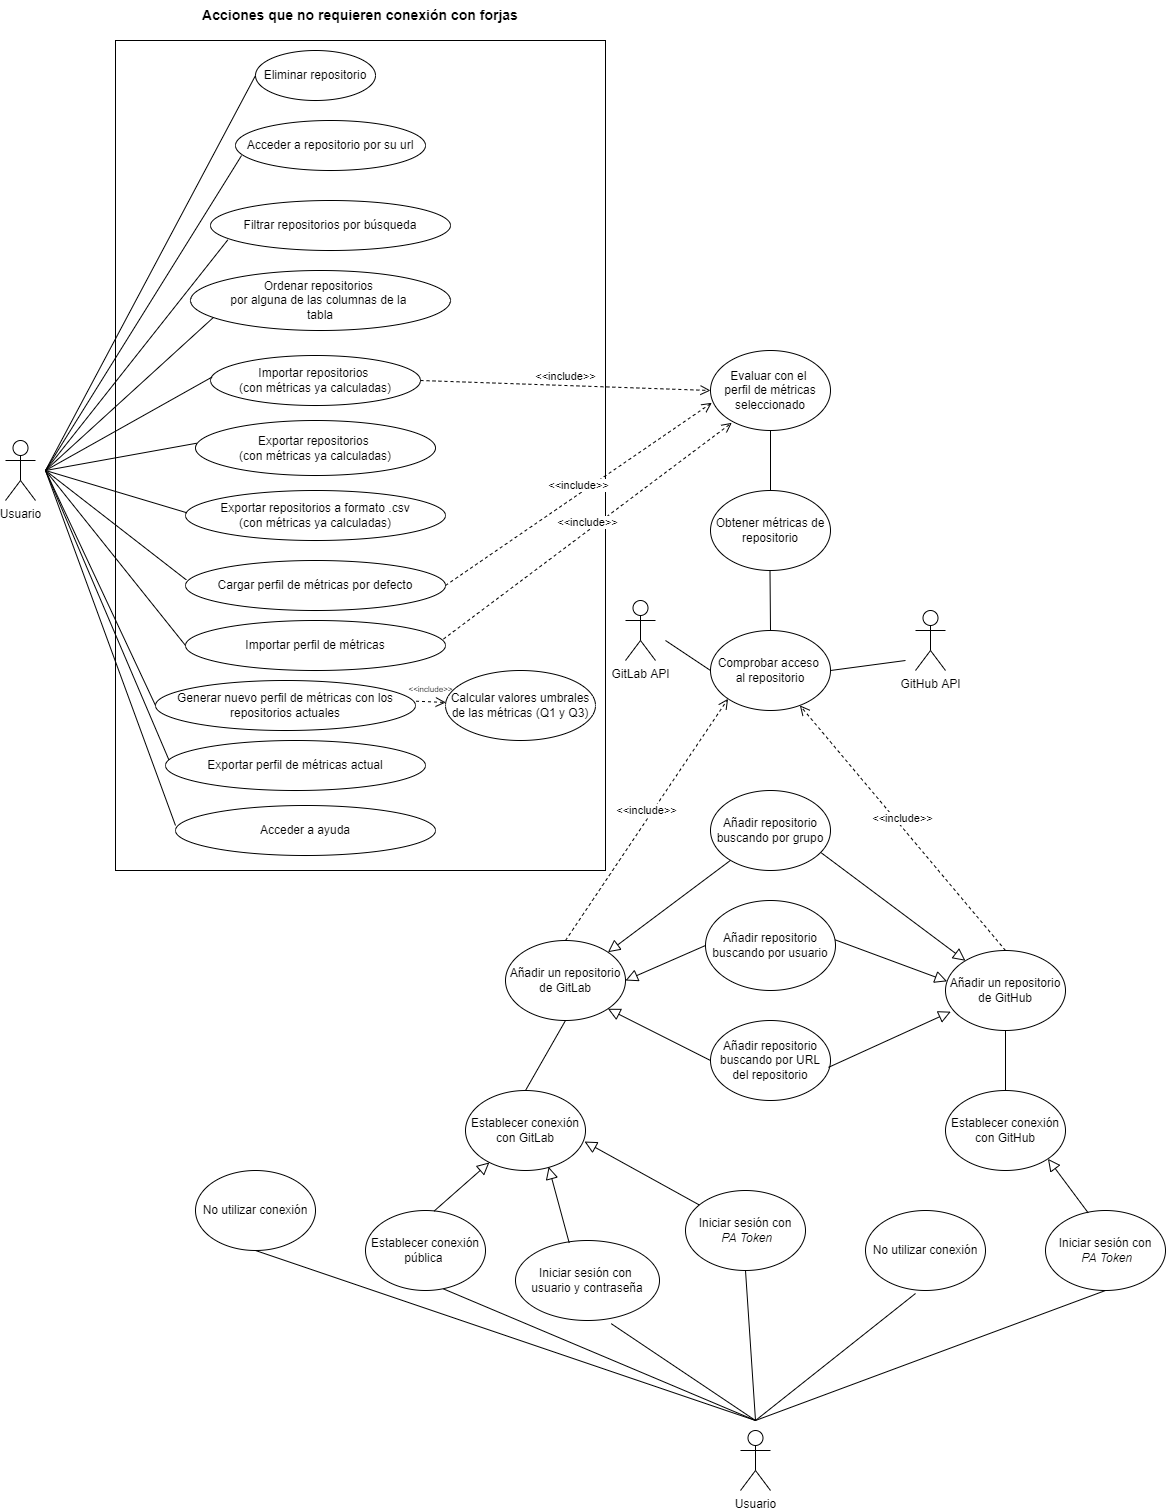
\includegraphics[width=1\textwidth]{AnexC_Use_Cases}
	\caption{Diagrama de casos de uso del proyecto}
	\label{fig:AnexC_Use_Cases}
\end{figure}
\FloatBarrier

A continuación se van a detallar los diferentes casos de uso por medio de tablas \cite{TFMANVIRECO} descriptivas:

\casoDeUso{
	CU-01
}{
	Establecer conexión con \textit{GitHub}
}{
	\tablaCasoDeUso{
		1.0
	}{
		RF-1, RF-1.1, RF-1.2, RF-1.3, RF-1.4
	}{
		Permite al usuario establecer una conexión con \textit{GitHub} para posteriormente poder importar repositorios y calcular sus métricas.
	}{
		Situado en la página principal.
	}{
		1 & Pulsar el botón de conexión con \textit{GitHub}. \\
		2 & Pulsar el botón \textit{Connect} en el diálogo de estado de la conexión. \\
		3 & Rellenar el \textit{input} del \textit{Personal Access Token} y pulsar el botón \textit{Connect} en el diálogo de conexión.
	}{
		Se ha establecido una conexión con \textit{GitHub} que permite importar repositorios de esta forja.
	}{
		1 & No se pulsa el botón \textit{Connect} en el diálogo de estado de la conexión. \\
		2 & Se selecciona el botón \textit{Don't connect} en el diálogo de conexión. \\
		3 & No se introduce un \textit{Personal Access Token} válido.
	}{Alta}{cu-01}
}

\casoDeUso{
	CU-02
}{
	Establecer conexión con \textit{GitLab}
}{
	\tablaCasoDeUso{
		1.0
	}{
		RF-2, RF-2.1, RF-2.2, RF-2.3, RF-2.4, RF-2.5, RF-2.6, RF-2.7
	}{
		Permite al usuario establecer una conexión con \textit{GitLab} para posteriormente poder importar repositorios y calcular sus métricas.
	}{
		Situado en la página principal.
	}{
		1 & Pulsar el botón de conexión con \textit{GitLab}. \\
		2 & Pulsar el botón \textit{Connect} en el diálogo de estado de la conexión. \\
		3.a & Rellenar los \textit{input} del \textit{Username} y \textit{Password} y pulsar el botón \textit{Connect} en el diálogo de conexión.  \\
		3.b & Seleccionar la opción \textit{Personal Access Token}, rellenar el \textit{input} del \textit{Personal Access Token} y pulsar el botón \textit{Connect} en el diálogo de conexión.\\
		3.c & Seleccionar la opción \textit{Public connection} y pulsar el botón \textit{Connect} en el diálogo de conexión.

	}{
		Se ha establecido una conexión con \textit{GitLab} que permite importar repositorios de esta forja.
	}{
		1 & No se pulsa el botón \textit{Connect} en el diálogo de estado de la conexión. \\
		2 & Se selecciona el botón \textit{Don't connect} en el diálogo de conexión. \\
		3.a & No se introducen un usuario y contraseña válidos. \\
		3.b & No se introduce un \textit{Personal Access Token} válido.
	}{Alta}{cu-02}
}

\casoDeUso{
	CU-03
}{
	Añadir un nuevo proyecto
}{
	\tablaCasoDeUso{
		1.0
	}{
		RF-3, RF-3.1, RF-3.1.1, RF-3.1.2, RF-3.1.3, RF-3.2, RF-3.3, RF-4, RF-4.2, RF-4.5, RF-4.6
	}{
		Añadir un nuevo proyecto para calcular sus métricas y evaluarlo.
	}{
		Se ha establecido una conexión.	
	}{
		1 & Pulsar el botón \textit{Project management}. \\
		2.a & Pulsar el botón \textit{Add new GitLab repository} en las opciones del desplegable. \\
		2.b & Pulsar el botón \textit{Add new GitHub repository} en las opciones del desplegable. \\
		3.a & Rellenar el input \textit{User ID or username}, seleccionar uno de los resultados del desplegable \textit{Project}.  \\
		3.b & Seleccionar la opción \textit{By Group}, rellenar el \textit{input} del \textit{Group ID or groupname}, seleccionar uno de los resultados del desplegable \textit{Project}. \\
		3.c & Seleccionar la opción \textit{By URL}, rellenar el input \textit{Project URL}. \\
		4 & Pulsar el botón \textit{Add}. \\
		5 & Se obtiene el proyecto y se calculan las métricas. \\
		6 & Se evalúan las métricas con el perfil de métricas seleccionado actualmente. \\
		7 & Se añade el proyecto al listado.
	}{
		Se ha añadido el proyecto al listado con sus métricas calculadas y evaluadas.
	}{
		1 & No se introducen un  \textit{User ID or username} o textit{Group ID or groupname} o bien \textit{Project URL} válidos. \\
		2 & La conexión establecida no tiene permisos suficientes para acceder al repositorio solicitado.  \\
		3 & Se intenta añadir un proyecto que ya está añadido previamente.
	}{Alta}{cu-03}
}


\casoDeUso{
	CU-04
}{
	Eliminar un proyecto
}{
	\tablaCasoDeUso{
		1.0
	}{
		RF-3.3
	}{
		Eliminar un proyecto del listado.
	}{
		Existe algún proyecto que eliminar.	
	}{
		1 & Pulsar el botón \textit{papelera} de la fila del listado correspondiente al proyecto que se desea eliminar. \\
		2 & El proyecto es eliminado del listado.
	}{
		El proyecto eliminado ya no está en el listado.
	}{
		1 & Se produce un error al eliminar el repositorio y éste permanece en el listado. 
	}{Baja}{cu-04}
}

\casoDeUso{
	CU-05
}{
	Volver a obtener métricas de un repositorio
}{
	\tablaCasoDeUso{
		1.0
	}{
		RF-3.5
	}{
		Permite volver a obtener las métricas de un repositorio ya añadido al listado.
	}{
		Se ha establecido una conexión a la forja origen del repositorio.
	}{
		1 & Pulsar el botón \textit{libro-calculadora} de la fila del listado correspondiente al proyecto que se desea actualizar. \\
		2 & Las métricas del proyecto son calculadas y evaluadas con el perfil actual. \\
	}{
		Las métricas del proyecto han sido calculadas y evaluadas con el perfil actual.
	}{
		1 & No existe conexión con la forja correspondiente. \\
		2 & La conexión actual no tiene permisos suficientes para obtener las métricas del repositorio.
	}{Baja}{cu-05}
}

\casoDeUso{
	CU-06
}{
	Exportar proyectos y métricas a formato `.emr'
}{
	\tablaCasoDeUso{
		1.0
	}{
		RF-3.6
	}{
		Permite exportar los proyectos y sus métricas ya calculadas en un formato que permite importación.
	}{
		Existen proyectos en el listado.
	}{
		1 & Pulsar el botón \textit{Project management}. \\
		2 & Pulsar el botón \textit{Export} del desplegable. \\
		3 & Pulsar el botón \textit{Download} del diálogo de confirmación. \\
		4 & Los repositorios y sus métricas son exportados en un archivo con formato `.emr'. \\
	}{
		Obtenemos un archivo que contiene la información de los repositorios y sus métricas en formato `.emr'.
	}{
		1 & No existen proyectos en el listado.
	}{Media}{cu-06}
}

\casoDeUso{
	CU-07
}{
	Exportar proyectos y métricas a formato `.csv'
}{
	\tablaCasoDeUso{
		1.0
	}{
		RF-3.7
	}{
		Permite exportar los proyectos y sus métricas ya calculadas en un formato que permite su uso por ejemplo en hojas de cálculo.
	}{
		Existen proyectos en el listado.
	}{
		1 & Pulsar el botón \textit{Project management}. \\
		2 & Pulsar el botón \textit{Export to CSV} del desplegable. \\
		3 & Pulsar el botón \textit{Download} del diálogo de confirmación. \\
		4 & Los repositorios y sus métricas son exportados en un archivo con formato `.csv'. \\
	}{
		Obtenemos un archivo que contiene la información de los repositorios y sus métricas en formato `.csv'.
	}{
		1 & No existen proyectos en el listado.
	}{Media}{cu-07}
}

\casoDeUso{
	CU-08
}{
	Importar proyectos desde archivo.
}{
	\tablaCasoDeUso{
		1.0
	}{
		RF-3.8, RF-3.9
	}{
		Permite importar una lista de proyectos con sus métricas desde un archivo con formato `.emr'.
	}{
		Existen proyectos en el listado.
	}{
		1 & Pulsar el botón \textit{Project management}. \\
		2 & Pulsar el botón \textit{Import} del desplegable. \\
		3.a & Pulsar el botón \textit{Upload File...} del diálogo de importación y seleccionar un archivo en el explorador de archivos. \\
		3.b & Soltar un fichero en la zona \textit{Drop file here}. \\
		4 & Si se detecta que ya hay repositorios con el mismo nombre, elegir si queremos sobreescrirlos o añadir sólo los que no estén. \\
		5 & Los repositorios del fichero y sus métricas son importados al listado y evaluados con el perfil actual. No se importa ningún proyecto que ya exista. \\
	}{
		Los repositorios del fichero y sus métricas son importados al listado y evaluados con el perfil actual, no se tiene ningún proyecto duplicado.
	}{
		1 & No se selecciona un archivo válido.
	}{Media}{cu-08}
}

\casoDeUso{
	CU-09
}{
	Filtrar proyectos.
}{
	\tablaCasoDeUso{
		1.0
	}{
		RF-3.10
	}{
		Permite filtrar los proyectos del listado por su nombre.
	}{
		Existen proyectos en el listado.
	}{
		1 & Escribir en el input \textit{Search} el texto a buscar. \\
		2 & En el listado sólo se mostrarán los proyectos que contengan dicho texto en su nombre.
	}{
		En el listado sólo se muestran los proyectos que contengan el texto buscado en su nombre.
	}{
		1 & No existen proyectos en el listado.	
	}{Baja}{cu-09}
}


\casoDeUso{
	CU-10
}{
	Ordenar proyectos.
}{
	\tablaCasoDeUso{
		1.0
	}{
		RF-3.11, RF-3.12
	}{
		Permite ordenar los proyectos por nombre, fecha o cualquiera de las métricas.
	}{
		Existen proyectos en el listado.
	}{
		1 & Hacer \textit{click} sobre el icono de ordenación de la columna por la que se desea ordenar (ascendente). \\
		2 & Volver a hacer \textit{click} si se desea cambiar a ordenación descendente. \\
		2 & Volver a hacer \textit{click} si se cancelar la ordenación. \\
		4 & Los proyectos de listado aparecen ordenados según la columna y criterio seleccionados.
	}{
		En el listado sólo se muestran los proyectos ordenados por la columna seleccionada y en el orden seleccionado.
	}{
		1 & No existen proyectos en el listado.	
	}{Baja}{cu-10}
}

\casoDeUso{
	CU-11
}{
	Evaluar con nuevo perfil de métricas
}{
	\tablaCasoDeUso{
		1.0
	}{
		RF-4.3
	}{
		Permite generar un perfil de métricas con los proyectos existentes en el listado y evaluarlos con el mismo.
	}{
		Existen proyectos en el listado.
	}{
		1 & Pulsar el botón \textit{Evaluate projects}. \\
		2 & Pulsar el botón \textit{Evaluate with new profile} del desplegable. \\
		3 & Los proyectos del listado son evaluados con el nuevo perfil generado a partir de ellos.
	}{
		Los proyectos del listado han sido evaluados con el nuevo perfil generado a partir de ellos.
	}{
		1 & No existen proyectos en el listado.	
	}{Alta}{cu-11}
}

\casoDeUso{
	CU-12
}{
	Exportar perfil de métricas
}{
	\tablaCasoDeUso{
		1.0
	}{
		RF-4.4
	}{
		Permite exportar el perfil de métricas actual en formato `.emr', éste es importable.
	}{
		Existen proyectos en el listado.
	}{
		1 & Pulsar el botón \textit{Evaluate projects}. \\
		2 & Pulsar el botón \textit{Export actual profile} del desplegable. \\
		3 & Pulsar el botón \textit{Download} del diálogo \textit{Export metric profile}. \\
		4 & El perfil de métricas actual es exportado.
	}{
		Obtenemos un fichero en formato `.emr' que contiene la información del perfil actual de métricas.
	}{
		1 & No existen proyectos en el listado.	
	}{Alta}{cu-12}
}

\casoDeUso{
	CU-13
}{
	Importar perfil de métricas
}{
	\tablaCasoDeUso{
		1.0
	}{
		RF-4.5
	}{
		Permite importar un perfil de métricas desde un archivo en formato `.emr'.
	}{
		Existen proyectos en el listado.
	}{
		1 & Pulsar el botón \textit{Evaluate projects}. \\
		2 & Pulsar el botón \textit{Evaluate with imported profile} del desplegable. \\
		3.a & Pulsar el botón \textit{Upload File...} del diálogo de importación y seleccionar un archivo en el explorador de archivos. \\
		3.b & Soltar un fichero en la zona \textit{Drop file here}. \\
		4 & El perfil de métricas es importado y los proyectos son evaluados con el.
	}{
		Se ha cargado un nuevo perfil de métricas y los proyectos del listado son evaluados con él.
	}{
		1 & No se ah seleccionado un archivo válido	
	}{Alta}{cu-13}
}
\apendice{Especificación de diseño}\label{anex:C}

\section{Introducción}
En este apartado recogen las causas por las que se han adoptado las soluciones de diseño del software desarrollado, divididas diseño de datos, arquitectónico y diseño de la interfaz de usuario.

\section{Diseño de datos}\label{sec:C_2}
Las entidades con las que se trabaja en el proyecto son clases de Java. Si en un futuro se trabajase con una base de datos se podrían convertir las entidades de ésta a las clases Java que se utilizan actualmente sin mayor problema.

En el paquete \ruta{datamodel} podemos encontrar las clases más importantes en relación a los datos:
\begin{itemize}
	\item \ruta{Repository}. Sirve como definición de los datos que se obtienen de un repositorio. Estos datos son:
	\begin{itemize}
		\item URL, nombre e ID del proyecto
		\item Métricas internas (\ruta{RepositoryInternalMetrics}). Representan los valores de los que se obtienen las métricas externas y que interesan para satisfacer los requisitos funcionales de la aplicación.
		\item Resultados de las métricas (\ruta{MetricsResults}). Al añadir un repositorio estos se calcularán y quedarán almacenados en una instancia de esta clase.
		\item Evaluación del proyecto (\textit{projectEvaluation}). En esta clase se evalúan las diferentes métricas en función de sus umbrales y se almacena el porcentaje de métricas evaluadas como `buenas' cada vez que se calcule alguna de ellas.
		\item Cabe indicar que se ha definido la igualdad de los repositorios en base a su URL, ID y nombre.

	\item \ruta{RepositoryInternalMetrics}. Esta clase contiene toda la información de un repositorio necesaria para calcular las métricas, que es la fecha de medición, el número total de issues, el número total de commits, el número de issues cerradas, una colección de días que se tardan en cerrar las issues, otra colección con las fechas de los commits, el tiempo de vida del proyecto, una colección de los \textit{jobs} del proyecto y una colección de las \textit{releases} del proyecto. \\
	Cabe indicar que se define el método \textit{equals} a partir de la fecha de medición.
	\item \ruta{User}. Sirve para almacenar información que se obtiene de las forjas de repositorios acerca del usuario que ha iniciado sesión. Se almacenan la ID de usuario, la URL del avatar, el e-mail, el nombre y el nombre de usuario.
	\end{itemize}
	\item Se han implementado clases personalizadas para envolver a las clases relacionadas con los \textit{jobs} del proyecto y una colección de las \textit{releases} devueltas por las librerías de integración con las forjas de repositorios. Esto ha sido necesario ya que las clases obtenidas por medio de las librerías de conexión no son serializables y en la aplicación necesitamos serializar los resultados de las métricas para poder exportarlos e importarlos.\\
	Las clases generadas son: \textit{CustomGithubApiJob}, \textit{CustomGithubApiRelease}, \textit{CustomGitlbApiJob} y \textit{CustomGitlabApiRelease}.\\
	Hay que indicar que en estas clases se han de almacenar como variables aquellas que se tengan que usar para los calculos de las métricas, por ejemplo el nombre de los \textit{jobs} con \textit{this.job = job.getName()} para el cálculo de la métrica IC3.
\end{itemize}
	
\section{Diseño arquitectónico}
A continuación se describe la estructura de paquetes del proyecto y las clases que contienen.

\subsection{Paquete repositorydatasource}
El paquete define el framework de conexión a una forja de repositorios e implementa la conexión a GitLab.

\imagen{AnexC_RepositoryDataSource}{Paquete repositorydatasource}

Para crear un \textit{Repositorydatasource} con acceso a otra forja solo se tiene que implementar las dos interfaces, sin necesidad de hacer más cambios en el código, como se puede ver en la imagen la implementación para GitHub y GitLab es equivalente.

\subsection{Paquete metricsengine}
En este paquete se define el framework de medición y sigue el diseño descrito en \textit{Soporte de Métricas con Independencia del Lenguaje para la Inferencia de Refactorizaciones} \cite{marticorena_sanchez_soporte_2005}, con unos pequeños cambios:

\begin{itemize}
	\tightlist
	\item Se ha aplicado a las métricas concretas el patrón \textit{\textbf{Singleton}} \footnote{\url{https://refactoring.guru/design-patterns/singleton}}, que obliga a que solo haya una única instancia de cada métrica. Además, se ha aplicado el patrón \textit{\textbf{Método fábrica}} \footnote{\url{https://refactoring.guru/design-patterns/factory-method}} tal y como se muestra en la Fig. \ref{fig:M3_CambiosFrameworkMedicion1}, de forma que \textit{MetricConfiguration} no esté asociada con la métrica en sí, sino con una forma de obtenerla.\\
	El objetivo de trabajar de esta manera es facilitar la persistencia de un perfil de métricas. Las métricas se podrían ver como clases estáticas, no varían en tiempo de ejecución y solo debería haber una instancia de cada una de ellas. Por ello, al importar o exportar un perfil de métricas con su conjunto de configuraciones de métricas, estas configuraciones no deberían asociarse a la métrica, sino a la forma de acceder a la única instancia de esa métrica. 
	\item Se trabaja con los métodos \textit{evaluate} y \textit{getEvaluationFunction} en la interfaz \textit{IMetric}, ver Fig. \ref{fig:M3_CambiosFrameworkMedicion2}, para obtener los valores de las mismas, siendo estos métodos un añadido que se realizó al framework de medición original.\\
	Esto permite interpretar y evaluar los valores medidos sobre los valores límite de la métrica o configuración de métrica deduciéndose si su valor es bueno o no según el perfil de evaluación.\\
	 Por ejemplo, puede que para unas métricas un valor aceptable esté comprendido entre el valor límite superior y el valor límite inferior; y para otras un valor aceptable es aquel que supere el límite inferior.\\
	\textit{EvaluationFunction} es una interfaz funcional \footnote{Enlaces a la documentación: \url{https://docs.oracle.com/javase/8/docs/api/java/lang/FunctionalInterface.html} --- \url{https://docs.oracle.com/javase/8/docs/api/java/util/function/package-summary.html}} 
	de tipo `\textit{función}': recibe uno o más parámetros y devuelve un resultado. Este tipo de interfaces son posibles a partir de la versión 1.8 de Java.\\
	Esto permite definir los tipos de los parámetros y de retorno de una función que se puede almacenar en una variable. De este modo se puede almacenar en una variable la forma en la que se puede evaluar la métrica.
\end{itemize}

\imagen{M3_CambiosFrameworkMedicion1}{Patrones ``singleton'' y ``método fábrica'' sobre el framework de medición}

\imagen{M3_CambiosFrameworkMedicion2}{Añadido al framework de medición la evaluación de métricas}

\subsection{Paquete gui}
En este paquete se define toda la interfaz gráfica.


\subsection{Paquete exceptions}
En este paquete se encuentran las excepciones de la aplicación, además se trabaja con códigos de error y mensajes para poder ser identificados y comprendidos en el logger fácilmente. Se ha creado un diseño en el que, para definir nuevas excepciones, se puede extender de \textit{ApplicationException}, copiar y adaptar los constructores y modificar con \textit{@Override} el método \textit{generateMessage()} con los mensajes personalizados en un \textit{switch} para cada código de error:

\begin{figure}[!h]
	\centering
	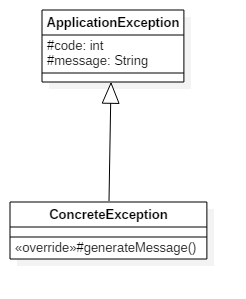
\includegraphics[width=0.5\textwidth]{AnexC_Exceptions}
	\caption{Paquete exceptions}\label{fig:AnexC_Exceptions}
\end{figure}
\FloatBarrier

Trabajando con este diseño se han podido implementar excepciones para las nuevas métricas.

\subsection{Paquete datamodel}
El paquete datamodel contiene las diferentes clases que se han descrito anteriormente en la sección \ref{sec:C_2}. Si en un futuro se integraran nuevas forjas de repositorios puede que sea necesario añadir nuevas clases de envoltura para serializar los valores que obtengamos como se ha visto anteriormente.

\subsection{Paquete app}
Contiene las clases que sirven de conexión entre la interfaz de usuario y la lógica de la aplicación.

\begin{figure}[!h]
	\centering
	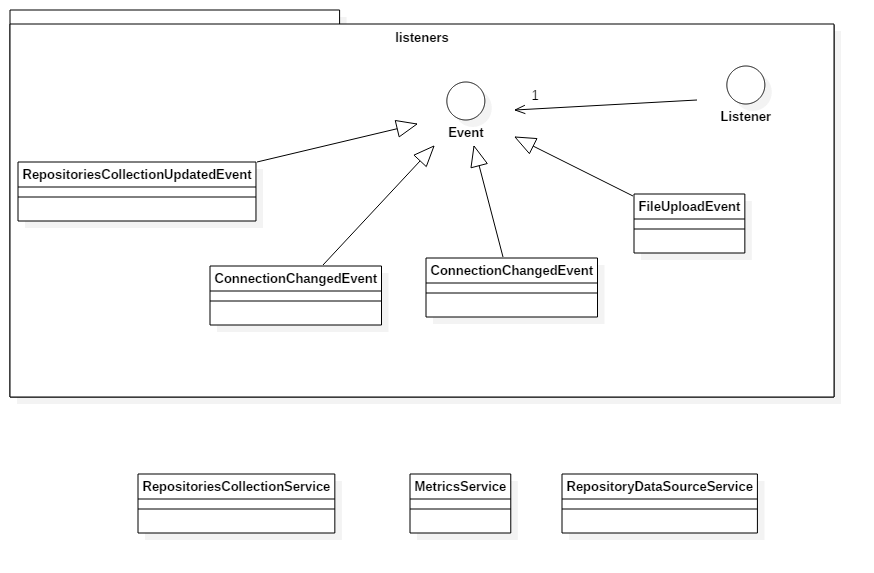
\includegraphics[width=0.7\textwidth]{AnexC_app}
	\caption{Paquete app}\label{fig:AnexC_app}
\end{figure}
\FloatBarrier

Las clases que encontramos en este paquete son:

\begin{description}
	\item[MetricsService] Define una fachada de conexión entre el motor de métricas y el resto de componentes.
	\item[RepositoriesCollectionService] Se encarga de almacenar los repositorios en una colección
	\item[RepositoriesCollectionService] Define una fachada entre la fuente de datos (\textit{repositorydatasource}) y el resto de componentes.
\end{description}

\subsubsection{Paquete app.listeners}
En este paquete trabajamos con el patrón observador. Se definen la interfaz \textit{Listener} y la interfaz \textit{Event} y se implementan algunos eventos como el de conexión a una forja o el de subida de un archivo para realizar diferentes acciones cuando se den dichos eventos.\\ 
La interfaz \textit{Event} sirve para implementar eventos a partir de ella, estos eventos normalmente tienen información relativa al suceso que ocurre. Por ejemplo, \textit{CurrentMetricProfileChangedEvent} contiene información sobre un cambio de perfil de métricas: el viejo perfil y el nuevo. La interfaz \textit{Listener} define una función a la que se le pasa un evento y sirve como interfaz funcional para ejecutar una acción (función lambda) que recibe por parámetro el evento.

\apendice{Documentación técnica de programación}\label{anex:D}

\section{Introducción}
En este documento de tratan diferentes aspectos técnicos de programación.

\section{Estructura de directorios}
En el proyecto el código fuente presenta la siguiente estructura:
\begin{itemize}
	\tightlist
	\item \ruta{/.gitignore}. Contiene los ficheros y directorios que el repositorio git no tendrá en cuenta
	\item \ruta{/.github/workflows/maven.yml}. Contiene los \textit{jobs} a ejecutar gracias a \textit{GitHub Actions} tras hacer un \textit{commit} o un \textit{merge} a la rama \textbf{main}. Permite y define la integración y el despliegue continuo.
	\item \ruta{/README.md}. Fichero que sirve de introducción al proyecto y que contiene información importante.
	\item \ruta{/pom.xml}. Fichero de configuración del proyecto \textit{Maven}.
	\item \ruta{/system.properties}. Fichero con propiedades del proyecto necesario para el despliegue en \textit{Heroku}.
	\item \ruta{/MemoriaProyecto}. Memoria del proyecto según la plantilla definida en \url{https://github.com/ubutfgm/plantillaLatex}.
	\item \ruta{/src/test/resources}. Datos almacenados en ficheros \textit{CSV} para proporcionar datos a test parametrizados.
	\item \ruta{/src/test/java}. Casos de prueba JUnit para la realización de pruebas. Se organiza de la misma forma que \ruta{/src/main/java}
	\item \ruta{/src/main/webapp/VAADIN/themes/MyTheme}. Tema principal utilizado por la aplicación el cual es generado por \textit{Vaadin}.
	\item \ruta{/src/main/webapp/frontend}. Fichero \textit{.css} y los diferentes iconos utilizado por la interfaz gráfica.
	\item \ruta{/src/main/webapp/images}. Imágenes que se muestran en la interfaz gráfica.
	\item \ruta{/src/main/resources}. Ficheros de configuración de la aplicación. En este caso el fichero log4j2.properties para configurar el sistema de logging.
	\item \ruta{/src/main/java}. Contiene todo el código fuente.
	\item \ruta{/src/main/java/app/}. Contiene fachadas que conectan la interfaz de usuario con el resto de componentes que componen la lógica de la aplicación.
	\item \ruta{/src/main/java/app/listeners}. Contiene observadores y eventos utilizados por la aplicación.
	\item \ruta{/src/main/java/datamodel}. Contiene las clases que representan el modelo de datos de la aplicación.
	\item \ruta{/src/main/java/exceptions}. Contiene excepciones definidas en la aplicación.
	\item \ruta{/src/main/java/gui}. Contiene la interfaz de usuario.
	\item \ruta{/src/main/java/gui/views}. Contiene páginas y componentes de \textit{Vaadin} que componen la interfaz gráfica de la aplicación.
	\item \ruta{/src/main/java/metricsengine}. Contiene el motor de métricas.
	\item \ruta{/src/main/java/metricsengine/numeric\_value\_metrics}. Métricas definidas y sus respectivas fábricas (Patrón de diseño método fábrica\footnote{https://refactoring.guru/design-patterns/factory-method}). Todas las métricas tienen resultados numéricos.
	\item \ruta{/src/main/java/metricsengine/values}. Valores que devuelven las métricas.
	\item \ruta{/src/main/java/repositorydatasource}. \textit{Framework} de conexión a las diferentes forjas de repositorios como \textit{GitHub} o \textit{GitLab}.
\end{itemize}

\newpage
\section{Manual del programador}
En este apartado se tratan algunas bases para entender como continuar trabajando en las diferentes implementaciones de la aplicación y los posibles puntos donde trabajar.

\subsection{\textit{Framework} de conexión}
El \textit{framework} de conexión a una forja de repositorios (como \textit{GitHub}) está definido en el paquete \textit{repositorydatasource}. Consta de dos interfaces, la más importante es la interfaz \textit{RepositoryDataSource}.

En el Anexo C, se muestra un diagrama de clases en la Fig. \ref{fig:AnexC_RepositoryDataSource}. El paquete \textit{repositorydatasource} consta de dos interfaces que se han de implementar de forma particular para cada forja para así conectar el \textit{API} de la forja de repositorios con el resto de la aplicación. \\
Una solo es una fábrica que sirve instanciar un \textit{RepositoryDataSource} como por ejemplo \textit{RepositoryDataSourceUsingGithubAPI}.\\ Esta última es la que contiene las funciones para establecer una conexión y obtener los datos de los repositorios. Una vez tengamos implementadas estas interfaces para una nueva forja de repositorios se tiene que cambiar la llamada a la fábrica a la nueva, por ejemplo:

\begin{minipage}{\linewidth}
\tiny \begin{verbatim}
...
public class RepositoryDataSourceFactoryGithub implements RepositoryDataSourceFactory {

	@Override
	public RepositoryDataSource getRepositoryDataSource() {
		return RepositoryDataSourceUsingGithubAPI.getGithubRepositoryDataSource();
	}

}
...
\end{verbatim}
\end{minipage}	

\subsection{Motor de métricas}
El motor de métricas se implementó con una base inicial a una solución propuesta en \textit{Soporte de Métricas con Independencia del Lenguaje para la Inferencia de Refactorizaciones} \cite{marticorena_sanchez_soporte_2005}. El diseño se puede observar en las figuras Fig. \ref{fig:M3_CambiosFrameworkMedicion1} y Fig. \ref{fig:M3_CambiosFrameworkMedicion2}.
\imagen{MCTMotorMetricas}{Diagrama del \textit{framework} para el cálculo de métricas con perfiles.}

Trabajando con este diseño se han podido implementar las nuevas métricas relacionadas con la Integración y Despliegue continuos (\textit{CICD}) y de la misma manera se podrían añadir más métricas a al proyecto.

\newpage
\section{Compilación, instalación y ejecución del proyecto}
Para compilar el proyecto es necesario tener \textit{Java 11} y \textit{Maven} 3.6.0 o superior instalados en el equipo. Para ambas herramientas, el proceso de instalación es el mismo: descomprimir un archivo en la carpeta que se desee, configurar las variables de entorno del sistema \textit{JAVA\_HOME} y  \textit{CATALINA\_HOME} apuntando a los directorios de instalación que contienen la carpeta \ruta{bin}, y añadir al \textit{PATH} del sistema la ruta hacia los directorios \ruta{bin}.\\

Una vez instalados \textit{Java} y \textit{Maven}, para compilar se utilizaría el comando \ruta{mvn install} desde el directorio raíz del proyecto.\\

Para ejecutar el proyecto en nuestra máquina utilizando \textit{Jetty} (nos ayuda al detectar automáticamente cambios en el código y recompilando automáticamente) basta con ejecutar: \ruta{mvn jetty:run} tras haber instalado la aplicación con \textit{Maven}.\\

Para generar un .war compilando la aplicación es necesario hacerlo en modo producción, para ello ejecutaremos: \ruta{mvn clean package -Pproduction}.\\

Por último, para desplegar la aplicación desde la consola (si no tenemos configurado el despliegue continuo), tendremos que ejecutar:
\ruta{heroku login} o bien \ruta{winpty heroku.cmd login }\\
Hacer \textit{login} en \textit{Heroku} con el navegador y tras esto ejecutar:\\
\ruta{heroku war:deploy target/[\textit{nombre-de-la-aplicación}]-[versión].war --app [\textit{nombre-de-la-aplicación-en-Heroku}]}\\

\newpage
\section{Pruebas del sistema}
Se ha generado una batería de pruebas en \ruta{src/test/java}. Algunos de estos test son parametrizados y los valores se encuentran en ficheros \textit{.csv} en la carpeta \ruta{src/test/resources}.

Para ejecutar las pruebas y obtener informes de cobertura de código podemos hacerlo desde el \textit{IDE Eclipse} (\textit{Coverage As} -> \textit{JUnit Test} o bien desde consola corriendo:\\
\ruta{mvn jacoco:report}\\
o si lo necesitamos inicialmente:\\
\ruta{mvn clean jacoco:prepare-agent install jacoco:report}

\apendice{Documentación de usuario}

\section{Introducción}

\section{Requisitos de usuarios}

\section{Instalación}

\section{Manual del usuario}





\bibliographystyle{plain}
\bibliography{bibliografiaAnexos}

\end{document}
